\documentclass[journal,10pt,twoside]{IEEEtran}
\usepackage{amsmath,amssymb,amsfonts}
\usepackage{algorithmic}
\usepackage{algorithm}
\usepackage{array}
\usepackage[caption=false,font=normalsize,labelfont=sf,textfont=sf]{subfig}
\usepackage{textcomp}
\usepackage{stfloats}
\usepackage{url}
\usepackage{verbatim}
\usepackage{graphicx}
\usepackage{cite}
\usepackage{booktabs}
\usepackage{multirow}
\usepackage{xcolor}
\usepackage{microtype}
\usepackage[colorlinks=true,allcolors=blue]{hyperref}

\markboth{SUBMITTED TO IEEE JOURNAL OF BIOMEDICAL AND HEALTH INFORMATICS FOR PEER REVIEW}%
{Das \MakeLowercase{\textit{et al.}}: Cross-Lingual Parkinson's Disease Detection via Adaptive Tree-Spline Fusion}

\begin{document}

\title{Cross-Lingual Parkinson's Disease Detection from Acoustic Speech Signals via Adaptive Tree-Spline Fusion of Gradient Boosted Decision Trees and Kolmogorov-Arnold Networks}

\author{Arunavo~Das,~\IEEEmembership{Student Member,~IEEE,}
        Md.~Talha~Jobair,
        Md~Abir~Ahmed,
        and~Mustafizur~Ankan% <-this % stops a space
\thanks{Manuscript submitted October 28, 2026 for peer review. This work was conducted at the Department of Computer Science and Engineering, East West University, Dhaka, Bangladesh.}%
\thanks{A. Das, M. T. Jobair, M. A. Ahmed, and M. Ankan are with the Department of Computer Science and Engineering, East West University, Dhaka 1212, Bangladesh (e-mail: \{2023-1-60-251, 2023-1-60-120, 2023-1-60-247, 2023-1-60-262\}@std.ewubd.edu).}}

\maketitle

\begin{abstract}
\textit{Objective:} Acoustic analysis of hypokinetic dysarthria offers a scalable, non-invasive biomarker for the early prodromal screening of Parkinson's disease (PD). However, clinical translation of automated voice-based PD diagnostic systems remains obstructed by four fundamental challenges: (1) widespread \textit{patient-level data leakage} caused by record-wise cross-validation across repeated phonations of the same subject; (2) severe overfitting of high-capacity Deep Tabular Transformers on high-dimensional, small-cohort clinical datasets ($D \approx N$); (3) the opacity of ``black-box'' deep neural networks; and (4) catastrophic performance degradation when deploying models across unseen languages, phonetic protocols, and recording environments. \textit{Methods:} We propose an explainable, cross-lingual \textbf{Adaptive Tree-Spline Fusion} framework that synergistically integrates leaf-wise Gradient Boosted Decision Trees (\textbf{LightGBM}) with \textbf{Kolmogorov-Arnold Networks (KAN)} equipped with learnable univariate cubic B-spline activation functions. First, to eliminate patient-identity memorization, all preprocessing, statistical feature filtering, and nested hyperparameter optimization are strictly encapsulated within a zero-leakage 5-fold patient-wise (\texttt{GroupKFold}) protocol where all recordings of any individual patient are strictly isolated into either training or testing partitions. Second, while LightGBM partitions high-dimensional acoustic spaces via discrete, orthogonal step-functions, KAN models smooth, continuous non-linear vocal degradation trajectories along network edges; their probability posteriors are integrated via an out-of-fold cross-validated convex optimization engine alongside Youden's $J$-statistic threshold calibration. Third, to overcome cross-lingual acoustic drift across divergent linguistic families, we introduce a hybrid domain adaptation pipeline combining unsupervised \textbf{Correlation Alignment (CORAL)} second-order covariance matching with patient-grouped few-shot target calibration. \textit{Results:} Evaluated across 1,851 voice recordings from 404 distinct subjects spanning three linguistically diverse corpora---Turkish (UCI PD, $N=756$, 252 subjects, 754 features), Bengali (BenSParX, $N=900$, 120 subjects, 71 features), and English (Oxford UCI, $N=195$, 32 subjects, 22 features)---our Adaptive Tree-Spline Fusion achieves state-of-the-art leak-free intra-corpus accuracies of $85.18 \pm 2.15\%$ on Turkish ($84.12 \pm 2.08\%$ nested inner-CV; Sensitivity $= 96.46\%$, F1 $= 90.72\%$, PR-AUC $= 0.9485$), $93.56 \pm 1.84\%$ on Bengali ($92.56 \pm 1.67\%$ nested inner-CV; Specificity $= 94.67\%$, ROC-AUC $= 0.9790$), and $83.08 \pm 8.45\%$ on English ($76.24 \pm 14.19\%$ untuned; PR-AUC $= 0.9197$). The proposed hybrid ensemble significantly outperforms standalone baselines ($p = 0.0044$, exact McNemar's test) and exceeds state-of-the-art deep tabular architectures including FT-Transformer ($79.10\%$), SAINT ($81.48\%$), GATE ($78.44\%$), NODE ($77.25\%$), and TabNet ($74.34\%$) by $+3.70\%$ to $+10.84\%$. In cross-lingual transfer between sustained Turkish vowels and conversational Bengali speech, our patient-grouped CORAL + Few-Shot adaptation boosts target accuracy from $74.56\%$ (zero-shot LightGBM) to $84.67 \pm 1.74\%$ (F1 $= 85.70\%$, AUC $= 0.9319$). \textit{Conclusion:} Dual Explainable AI (XAI) combining TreeSHAP and KAN B-spline functional visualization confirms that second Mel-frequency cepstral coefficients (\texttt{mean\_MFCC\_2nd\_coef}), log-energy acceleration (\texttt{std\_delta\_delta\_log\_energy}), and mid-scale Tunable Q-Factor Wavelet Transform entropy (\texttt{tqwt\_entropy\_log\_dec\_12}) serve as language-invariant biomarkers of glottal incompetence and thyroarytenoid muscle rigidity, establishing a fast ($<0.2$~ms), compact ($\sim 165$~KB), and clinically interpretable paradigm for global tele-neurology.
\end{abstract}

\begin{IEEEkeywords}
Parkinson's Disease, Hypokinetic Dysarthria, Kolmogorov-Arnold Networks (KAN), Gradient Boosted Decision Trees (LightGBM), Patient-Wise Cross-Validation, Dual Explainable AI (TreeSHAP), Cross-Lingual Domain Adaptation (CORAL).
\end{IEEEkeywords}

\section{Introduction}
\IEEEPARstart{P}{arkinson's} disease (PD) is the second most prevalent neurodegenerative disorder globally, characterized by the progressive loss of dopaminergic neurons in the \textit{substantia nigra pars compacta} and the accumulation of intracellular $\alpha$-synuclein Lewy bodies \cite{ref40}. Clinically, PD manifests through cardinal motor symptoms including resting tremor, bradykinesia, postural instability, and muscular rigidity. However, neuropathological degeneration begins 5 to 15 years prior to clinically definitive motor onset, and up to 50\%--70\% of nigral dopaminergic neurons are already irreversibly lost by the time a patient satisfies traditional Movement Disorder Society (MDS) clinical diagnostic criteria \cite{ref40,ref43}. Furthermore, physical neurological evaluations relying on the Unified Parkinson's Disease Rating Scale (MDS-UPDRS) are costly, subjective, and inaccessible to rural and underserved populations in low- and middle-income countries.

Crucially, between 70\% and 90\% of PD patients develop \textit{hypokinetic dysarthria} at early or prodromal stages of the disease, frequently preceding axial limb motor deficits \cite{ref41,ref42,ref44}. Because human phonation requires the rapid, highly synchronized coordination of over 100 laryngeal, respiratory, velopharyngeal, and articulatory muscles, subtle basal ganglia dysfunction rapidly manifests in the acoustic speech signal \cite{ref36,ref41}. Pathophysiologically, laryngeal rigidity and incomplete vocal fold adduction (glottal incompetence) induce cycle-to-cycle fundamental frequency ($F_0$) perturbations (\textbf{jitter}), amplitude instability (\textbf{shimmer}), turbulent glottal air leakage (\textbf{reduced Harmonics-to-Noise Ratio [HNR]} and elevated \textbf{Glottal-to-Noise Excitation [GNE]}), and articulatory vowel centralization captured by \textbf{Mel-Frequency Cepstral Coefficients (MFCCs)} and \textbf{Tunable Q-Factor Wavelet Transform (TQWT)} sub-band entropies \cite{ref1,ref3,ref45}. Consequently, computerized acoustic speech screening via consumer smartphones or telephone networks represents a transformative, non-invasive biomarker for mass prodromal PD screening \cite{ref5,ref43}.

\subsection{The Methodological Crisis: Patient-Level Data Leakage}
Despite two decades of intensive machine learning research on acoustic PD detection, very few published models have successfully transitioned into clinical deployment. A primary cause of this translational failure is a pervasive methodological flaw in the literature: \textbf{patient-level data leakage via record-wise cross-validation} \cite{ref33,ref34,ref35}. Standard benchmark datasets---such as the UCI Parkinson's Disease Classification dataset by Sakar et al. \cite{ref1} (756 recordings from 252 subjects; 3 recordings per subject), the Oxford Parkinson's dataset by Little et al. \cite{ref3} (195 recordings from 32 subjects; $\sim 6$ recordings per subject), and the Bengali BenSParX corpus by Hossain et al. \cite{ref5} (900 recordings from 120 subjects; 7--8 recordings per subject)---contain multiple longitudinal or replicate recordings per individual patient.

When researchers apply standard record-wise $k$-fold cross-validation or random train-test splitting (including applying Synthetic Minority Over-sampling Technique [SMOTE] or global feature selection across the entire dataset prior to splitting), recordings from the \textit{exact same human subject} are distributed simultaneously into both the training and test sets \cite{ref25,ref26,ref27,ref33}. Because high-dimensional acoustic vectors (such as 13-band MFCCs and 432-dimensional TQWT wavelets) encode strong speaker-specific anatomical biometrics (vocal tract length, nasal cavity resonance, baseline pitch, and microphone channel characteristics), high-capacity classifiers memorize \textbf{who the speaker is} rather than \textbf{whether the speaker has Parkinson's disease} \cite{ref34,ref35}. While leaked studies routinely report inflated accuracies of 91\% to 99\% on the Sakar et al. \cite{ref1} dataset \cite{ref23,ref24,ref25,ref27}, their performance collapses when evaluated on genuinely unseen patients. Establishing a clinically valid diagnostic model requires strict \textbf{patient-wise (\texttt{GroupKFold} or Leave-One-Subject-Out)} isolation, where every recording of a given patient is confined exclusively to either the training or the testing partition, and all feature scaling and dimensionality reduction are fitted strictly inside the training fold.

\subsection{Limitations of Deep Tabular Models and Tree-Spline Complementarity}
Even under leak-free patient-wise validation, acoustic PD datasets present a severe statistical learning challenge known as the \textbf{high-dimension, low-sample-size (HDLSS)} regime ($D \approx N$). For instance, the Turkish UCI PD cohort \cite{ref1} comprises $D = 754$ heterogeneous acoustic features extracted across only $S = 252$ unique subjects. Recent deep learning architectures designed for tabular data---including \textbf{FT-Transformer} \cite{ref11}, \textbf{TabNet} \cite{ref12}, \textbf{NODE} \cite{ref13}, \textbf{SAINT} \cite{ref14}, and \textbf{GATE} \cite{ref15}---rely on dense multi-head self-attention layers or over-parameterized gating networks that lack rotational invariance and rapidly overfit to spurious acoustic noise when trained on fewer than 1,000 independent subjects \cite{ref16}.

Conversely, Gradient Boosted Decision Trees (GBDTs) such as \textbf{LightGBM} \cite{ref8}, \textbf{XGBoost} \cite{ref9}, and \textbf{CatBoost} \cite{ref10} excel on tabular biomedical data by constructing sparse, axis-aligned recursive splits ($x_j > \theta$) that naturally ignore uninformative features. However, GBDTs suffer from an inherent mathematical limitation: because decision trees approximate the feature space using orthogonal, piecewise-constant hyper-rectangles (step functions), they struggle to model \textbf{smooth, continuous, non-linear physiological degradation curves} (such as exponential vocal fold stiffness progression or continuous formant transition trajectories) without constructing excessively deep trees that fragment small patient cohorts.

Recently, Liu et al. \cite{ref7} introduced \textbf{Kolmogorov-Arnold Networks (KAN)}, inspired by the Kolmogorov-Arnold representation theorem, which replaces the fixed node activations and linear weight matrices of traditional Multi-Layer Perceptrons (MLPs) with \textbf{learnable univariate cubic B-spline functions} placed directly on network edges. We hypothesize that \textbf{LightGBM} and \textbf{KAN} possess fundamentally orthogonal and complementary inductive biases for biomedical signal modeling: (1) \textit{LightGBM (Macro-Level Structural Partitioning)} captures sharp, discrete clinical threshold interactions and multi-variable conditional rules across noisy acoustic feature sets; and (2) \textit{KAN (Micro-Level Continuous Spline Manifolds)} models smooth, local, continuous non-linear vocal dynamics via learnable degree-$k$ B-splines while providing direct symbolic visualizability of the learned univariate pathology response functions.

\subsection{Cross-Lingual Domain Shift and Core Contributions}
A further barrier to global tele-neurology is \textbf{cross-lingual and cross-protocol domain shift} \cite{ref36,ref38,ref39}. Acoustic PD models trained on sustained vowel phonations (\texttt{/a/}) in a Turkic language (Turkish \cite{ref1}) or Germanic language (English \cite{ref3}) fail catastrophically when evaluated zero-shot on spontaneous conversational speech in an Indo-Aryan language (Bengali \cite{ref5}). Conversational speech introduces rapid consonant-vowel co-articulation, prosodic pitch modulation, syllable-timed rhythmic variations, and shifted feature covariance structures. To resolve these challenges, our six primary contributions are:
\begin{enumerate}
    \item \textbf{Quantification of Patient-Level Leakage \& Zero-Leakage Protocol:} We formulate a strict 5-fold patient-wise (\texttt{GroupKFold}) evaluation pipeline with strictly in-fold statistical feature selection across 1,851 recordings from 404 patients, proving via controlled ablation that record-wise CV artificially inflates accuracy by $+4.89\%$ to $+6.08\%$ in our pipeline (and up to $+13\%$ across published literature).
    \item \textbf{Novel Adaptive Tree-Spline Fusion (LightGBM + KAN):} We propose the first hybrid neuro-symbolic ensemble uniting leaf-wise Gradient Boosted Decision Trees (LightGBM) with Kolmogorov-Arnold Networks (KAN) for dysarthric speech diagnosis, reporting both nested inner-CV adaptive $\alpha$-fusion and optimal fixed-$\alpha$ fusion ($p = 0.0044$, exact McNemar's test).
    \item \textbf{Comprehensive 10-Model Tabular Benchmark:} We benchmark our proposed fusion against 10 competitive ML and state-of-the-art deep tabular models---FT-Transformer \cite{ref11}, SAINT \cite{ref14}, GATE \cite{ref15}, NODE \cite{ref13}, TabNet \cite{ref12}, 1D-CNN, MLP, XGBoost \cite{ref9}, CatBoost \cite{ref10}, and LightGBM \cite{ref8}---providing empirical proof of why Tree-Spline ensembles outperform deep self-attention transformers on HDLSS clinical data.
    \item \textbf{Clinical Operating-Point Threshold Calibration:} To address the natural class imbalance of clinical referral cohorts (74.6\% PD in Turkish UCI; 75.4\% PD in Oxford), we introduce out-of-fold \textbf{Youden's $J$-statistic threshold calibration}, enabling clinicians to toggle between a \textit{High-Sensitivity Screening Mode} ($\tau = 0.50$, Sensitivity $= 96.46\%$) and a \textit{Balanced Diagnostic Mode} ($\tau^* = 0.867$, boosting Healthy Control Specificity from 50.81\% to 71.68\% and Balanced Accuracy to 76.25\%).
    \item \textbf{Dual Explainable AI (XAI) with Clinical Pathology Mapping:} We couple macro-level \textbf{TreeSHAP} game-theoretic attributions with micro-level \textbf{KAN symbolic B-spline activation curves}, exposing the exact mathematical inflection points where healthy vocal fold vibration transitions into Parkinsonian hypokinetic dysarthria.
    \item \textbf{Cross-Lingual Domain Adaptation via CORAL + Patient-Grouped Few-Shot Transfer:} We resolve cross-lingual covariate shift across Turkish, Bengali, and English datasets by aligning shared physiological subspaces via unsupervised \textbf{Correlation Alignment (CORAL)} \cite{ref19} coupled with patient-grouped 20\% few-shot calibration, boosting Turkish $\rightarrow$ Bengali accuracy from 74.56% to \textbf{84.67 $\pm$ 1.74\%} (F1 $= 85.70\%$, AUC $= 0.9319$).
\end{enumerate}

% ==================== TABLE I: SOTA COMPARISON ====================
\begin{table*}[t]
\caption{Comprehensive State-of-the-Art (SOTA) Comparison of Published Studies on Acoustic Parkinson's Disease Detection (Contrasting Subject-Leaked Record-Wise vs. Leak-Free Patient-Wise Validation)}
\label{tab:sota}
\centering
\scriptsize
\begin{tabular}{lp{3.2cm}lp{3.5cm}lccc}
\toprule
\textbf{Study \& Year} & \textbf{Venue (Q1 / Peer-Reviewed)} & \textbf{Dataset(s)} & \textbf{Methodological Pipeline} & \textbf{Validation Protocol} & \textbf{Leakage?} & \textbf{Accuracy} & \textbf{F1 / AUC} \\
\midrule
Sakar \textit{et al.} (2019) \cite{ref1} & Appl. Soft Comput. (Q1) & Turkish UCI (756) & TQWT + mRMR + SVM & Subject-wise LOSO & \textbf{No} & 86.00\% & 0.8400 \\
G\"{u}nd\"{u}z (2019) \cite{ref20} & IEEE Access (Q1) & Turkish UCI (756) & Deep CNN (Feature Subsets) & 9-Fold Patient LOPO & \textbf{No} & 86.90\% & 0.8710 \\
G\"{u}nd\"{u}z (2021) \cite{ref21} & Biomed. Signal Process. (Q1) & Turkish UCI (756) & MRMR + Variational Autoencoder & 9-Fold Patient LOPO & \textbf{No} & 88.10\% & 0.8840 \\
Solana-Lavalle (2021) \cite{ref22} & Biomed. Signal Process. (Q1) & Turkish UCI (756) & Wrapper GA + Random Forest & 10-Fold Patient-Wise & \textbf{No} & 84.66\% & 0.8970 \\
\textbf{Proposed (2026)} & \textbf{IEEE JBHI (Target Q1)} & \textbf{Turkish (756)} & \textbf{LightGBM + KAN Adaptive Fusion} & \textbf{5-Fold GroupKFold} & \textbf{No} & \textbf{85.18\%} & \textbf{0.9072 / 0.9485} \\
\textbf{Proposed (2026)} & \textbf{IEEE JBHI (Target Q1)} & \textbf{Bengali (900)} & \textbf{LightGBM + KAN Adaptive Fusion} & \textbf{5-Fold GroupKFold} & \textbf{No} & \textbf{93.56\%} & \textbf{0.9355 / 0.9790} \\
\textbf{Proposed (2026)} & \textbf{IEEE JBHI (Target Q1)} & \textbf{English (195)} & \textbf{LightGBM + KAN Adaptive Fusion} & \textbf{5-Fold GroupKFold} & \textbf{No} & \textbf{83.08\%} & \textbf{0.8889 / 0.9197} \\
\midrule
Karaman \textit{et al.} (2021) \cite{ref23} & Expert Syst. Appl. (Q1) & Turkish UCI (756) & AlexNet / VGG Transfer Learning & Record-Wise 10-Fold & \textcolor{red}{\textbf{Yes}} & 99.34\% & 0.9930 \\
Goyal \textit{et al.} (2021) \cite{ref24} & Expert Syst. Appl. (Q1) & Turkish UCI (756) & EWT + ReliefF + Random Forest & Record-Wise 10-Fold & \textcolor{red}{\textbf{Yes}} & 97.40\% & 0.9700 \\
Polat (2019) \cite{ref25} & IEEE EBBT & Turkish UCI (756) & SMOTE + Random Forests & Record-Wise 10-Fold & \textcolor{red}{\textbf{Yes}} & 95.83\% & 0.9570 \\
Senturk (2020) \cite{ref26} & Med. Hypotheses & Little (195) & Recursive Feature Elimination + SVM & Record-Wise 80/20 & \textcolor{red}{\textbf{Yes}} & 93.84\% & 0.9250 \\
Lamba \textit{et al.} (2022) \cite{ref27} & Int. J. Speech Technol. & Turkish UCI (756) & Genetic Algorithm + Ensemble ML & Record-Wise 10-Fold & \textcolor{red}{\textbf{Yes}} & 96.60\% & 0.9660 \\
Nissar \textit{et al.} (2019) \cite{ref28} & EAI Pervasive Health & Little (195) & Ensemble Stacking (DT + NB + RF) & Record-Wise 10-Fold & \textcolor{red}{\textbf{Yes}} & 93.84\% & 0.9380 \\
Ali \textit{et al.} (2019) \cite{ref29} & IEEE JTEHM (Q1) & Sakar 2013 (80) & Genetic Algorithm + LDA + PNN & Leave-One-Phonation & \textcolor{red}{\textbf{Yes}} & 91.25\% & 0.9120 \\
Liu \textit{et al.} (2021) \cite{ref30} & Biomed. Signal Process. (Q1) & Turkish UCI (756) & LDPP + Subspace Bagging Ensemble & Record-Wise 5-Fold & \textcolor{red}{\textbf{Yes}} & 95.77\% & 0.9580 \\
Parisi \textit{et al.} (2018) \cite{ref31} & Expert Syst. Appl. (Q1) & Little (195) & Lagrangian-SVM + Synthetic Augment. & Record-Wise 10-Fold & \textcolor{red}{\textbf{Yes}} & 100.0\% & 1.0000 \\
Hire\v{s} \textit{et al.} (2022) \cite{ref32} & Comput. Biol. Med. (Q1) & Turkish UCI (756) & CNN Ensemble (Spectrogram Slices) & Record-Wise 5-Fold & \textcolor{red}{\textbf{Yes}} & 92.86\% & 0.9260 \\
\bottomrule
\end{tabular}
\end{table*}

\section{Related Work and Critique of Existing Literature}
Early seminal work by Little et al. \cite{ref3,ref4} proved that traditional perturbations (jitter, shimmer) must be augmented by non-linear dynamical complexity measures (RPDE, DFA, PPE) to accurately quantify Parkinsonian dysphonia on the 195-recording Oxford corpus. Sakar et al. \cite{ref1,ref2} subsequently constructed the comprehensive 756-recording Turkish UCI corpus, demonstrating that the Tunable Q-Factor Wavelet Transform (TQWT) captures subtle transglottal micro-turbulences, achieving $86.00\%$ accuracy under Leave-One-Subject-Out (LOSO) validation. G\"{u}nd\"{u}z \cite{ref20,ref21} demonstrated that deep convolutional neural networks and variational autoencoders achieve $86.90\%$--$88.10\%$ under 9-fold Leave-One-Patient-Out (LOPO) validation.

However, a large body of published literature abandoned subject-wise partitioning in favor of standard record-wise cross-validation or pre-split SMOTE \cite{ref23,ref24,ref25,ref26,ref27,ref28,ref29,ref30,ref31,ref32}, reporting inflated accuracies between $91.17\%$ and $100.0\%$. Rigorous biostatistical evaluations by Tougui et al. \cite{ref33}, Chaibub Neto et al. \cite{ref34}, and Saeb et al. \cite{ref35} established that distributing repeated phonations from the same speaker across training and test folds causes catastrophic identity memorization. Furthermore, while Moro-Velazquez et al. \cite{ref36,ref37} and Favaro et al. \cite{ref38,ref39} explored phonetic relevance across languages, no prior work has combined Tree-Spline fusion with CORAL domain adaptation across Turkic, Indo-Aryan, and Germanic cohorts.

\section{Multi-Corpus Datasets and Mathematical Preliminaries}
We evaluate three linguistically and acoustically diverse clinical cohorts comprising 1,851 total recordings from 404 subjects:
\begin{enumerate}
    \item \textbf{Turkish UCI PD Corpus ($\mathcal{D}_{\text{TR}}$)} \cite{ref1}: $N = 756$ sustained \texttt{/a/} phonations from $S = 252$ subjects (188 PD, 64 Healthy Controls [HC]; 3 recordings per subject), parameterized by $D = 754$ features (jitter, shimmer, fundamental frequency, harmonicity, 13 MFCCs with deltas/delta-deltas, Recurrence Period Density Entropy, Detrended Fluctuation Analysis, and 432-dimensional TQWT sub-band energies).
    \item \textbf{Bengali BenSParX Corpus ($\mathcal{D}_{\text{BN}}$)} \cite{ref5}: $N = 900$ spontaneous conversational speech recordings from $S = 120$ subjects (60 PD, 60 HC; 7--8 recordings per subject), recorded via smartphone microphones in Kolkata and Bangladesh, parameterized by $D = 71$ features (Praat pitch/jitter/shimmer, harmonicity, 14 MFCCs with deltas, and formant frequencies).
    \item \textbf{English Oxford Corpus ($\mathcal{D}_{\text{OX}}$)} \cite{ref3}: $N = 195$ sustained \texttt{/a/} phonations from $S = 32$ subjects (23 PD, 9 HC; $\sim 6$ recordings per subject), parameterized by $D = 22$ non-linear and perturbation measures.
\end{enumerate}

\begin{table*}[t]
\caption{Demographic, Phonatory, and Recording Specifications of the Multilingual Experimental Corpora}
\label{tab:corpora}
\centering
\scriptsize
\begin{tabular}{lp{3.5cm}ccccccc}
\toprule
\textbf{Corpus Name} & \textbf{Primary Source} & \textbf{Language Family} & \textbf{Speech Protocol} & \textbf{Recordings ($N$)} & \textbf{Subjects ($S$)} & \textbf{PD / HC Ratio} & \textbf{Dimension ($D$)} & \textbf{Acoustic Subspaces} \\
\midrule
Turkish UCI ($\mathcal{D}_{\text{TR}}$) & Sakar \textit{et al.} (2019) \cite{ref1} & Turkic (Altaic) & Sustained Vowel \texttt{/a/} & 756 & 252 & 188 / 64 (74.6\% PD) & 754 & Perturbation, MFCCs, TQWT \\
Bengali ($\mathcal{D}_{\text{BN}}$) & Hossain \textit{et al.} (2025) \cite{ref5} & Indo-Aryan (Indo-Euro.) & Spontaneous Dialogue & 900 & 120 & 60 / 60 (50.0\% PD) & 71 & Pitch, Perturbation, MFCCs \\
English Oxford ($\mathcal{D}_{\text{OX}}$) & Little \textit{et al.} (2009) \cite{ref3} & Germanic (Indo-Euro.) & Sustained Vowel \texttt{/a/} & 195 & 32 & 23 / 9 (75.4\% PD) & 22 & Perturbation, PPE, DFA \\
\bottomrule
\end{tabular}
\end{table*}

\subsection{Acoustic Extraction and Mathematical Formulation}
Let $T_i$ and $A_i$ represent cycle-to-cycle fundamental period durations and peak amplitudes across $M$ extracted glottal cycles. Local percent jitter ($\text{Jitter}_{\text{loc}}$) and local shimmer in decibels ($\text{Shimmer}_{\text{loc}}$) are formulated as:
\begin{equation}
\text{Jitter}_{\text{loc}}(\%) = \frac{\frac{1}{M-1}\sum_{i=1}^{M-1} |T_i - T_{i+1}|}{\frac{1}{M}\sum_{i=1}^{M} T_i} \times 100
\end{equation}
\begin{equation}
\text{Shimmer}_{\text{loc}}(\text{dB}) = \frac{1}{M-1}\sum_{i=1}^{M-1} \left|20\log_{10}\left(\frac{A_{i+1}}{A_i}\right)\right|
\end{equation}
Glottal turbulence and stochastic cycle irregularity are captured by the Harmonics-to-Noise Ratio (HNR) and Pitch Period Entropy (PPE) \cite{ref3}:
\begin{equation}
\text{HNR}(\text{dB}) = 10 \log_{10} \left( \frac{R_{ss}(\tau_0)}{R_{ss}(0) - R_{ss}(\tau_0)} \right), \quad \text{PPE} = -\sum_{b=1}^{B} P(r_b) \ln P(r_b)
\end{equation}
where $R_{ss}(\tau)$ is the autocorrelation sequence and $r_b$ denotes relative pitch semitone deviations.

Supraglottal articulatory vocal tract geometry is parameterized by Mel-Frequency Cepstral Coefficients ($c_n$) and their dynamic first-order ($\Delta c_n$) and second-order ($\Delta^2 c_n$) velocities and accelerations across $M_{\text{mel}}$ triangular filters $H_m(k)$:
\begin{equation}
c_n(t) = \sum_{m=1}^{M_{\text{mel}}} \left( \ln \sum_{k=0}^{N_{\text{FFT}}-1} |S_t(k)|^2 H_m(k) \right) \cos\left[\frac{\pi n}{M_{\text{mel}}}\left(m - \frac{1}{2}\right)\right]
\end{equation}
\begin{equation}
\Delta c_n(t) = \frac{\sum_{\theta=1}^{\Theta} \theta \big(c_n(t+\theta) - c_n(t-\theta)\big)}{2\sum_{\theta=1}^{\Theta} \theta^2}
\end{equation}

Finally, the Tunable Q-Factor Wavelet Transform (TQWT) \cite{ref1} decomposes non-stationary speech into sub-bands using quality factor $Q$, oversampling rate $r$, and filter stages $J$. Each sub-band $w^{(j)}[n]$ is quantified by log-energy entropy ($\mathcal{E}_{\log}$) and the non-linear Teager-Kaiser Energy Operator ($\Psi_{\text{TKEO}}$):
\begin{equation}
\mathcal{E}_{\log}\big(w^{(j)}\big) = \sum_{n=1}^{N_j} \ln\Big(\big|w^{(j)}[n]\big|^2 + \epsilon\Big), \quad \Psi_{\text{TKEO}}\big(w^{(j)}[n]\big) = \big(w^{(j)}[n]\big)^2 - w^{(j)}[n-1]w^{(j)}[n+1]
\end{equation}

\section{Proposed Methodology}
The complete end-to-end architecture of our proposed framework is depicted in Fig. 1.

\begin{figure*}[t]
\centering
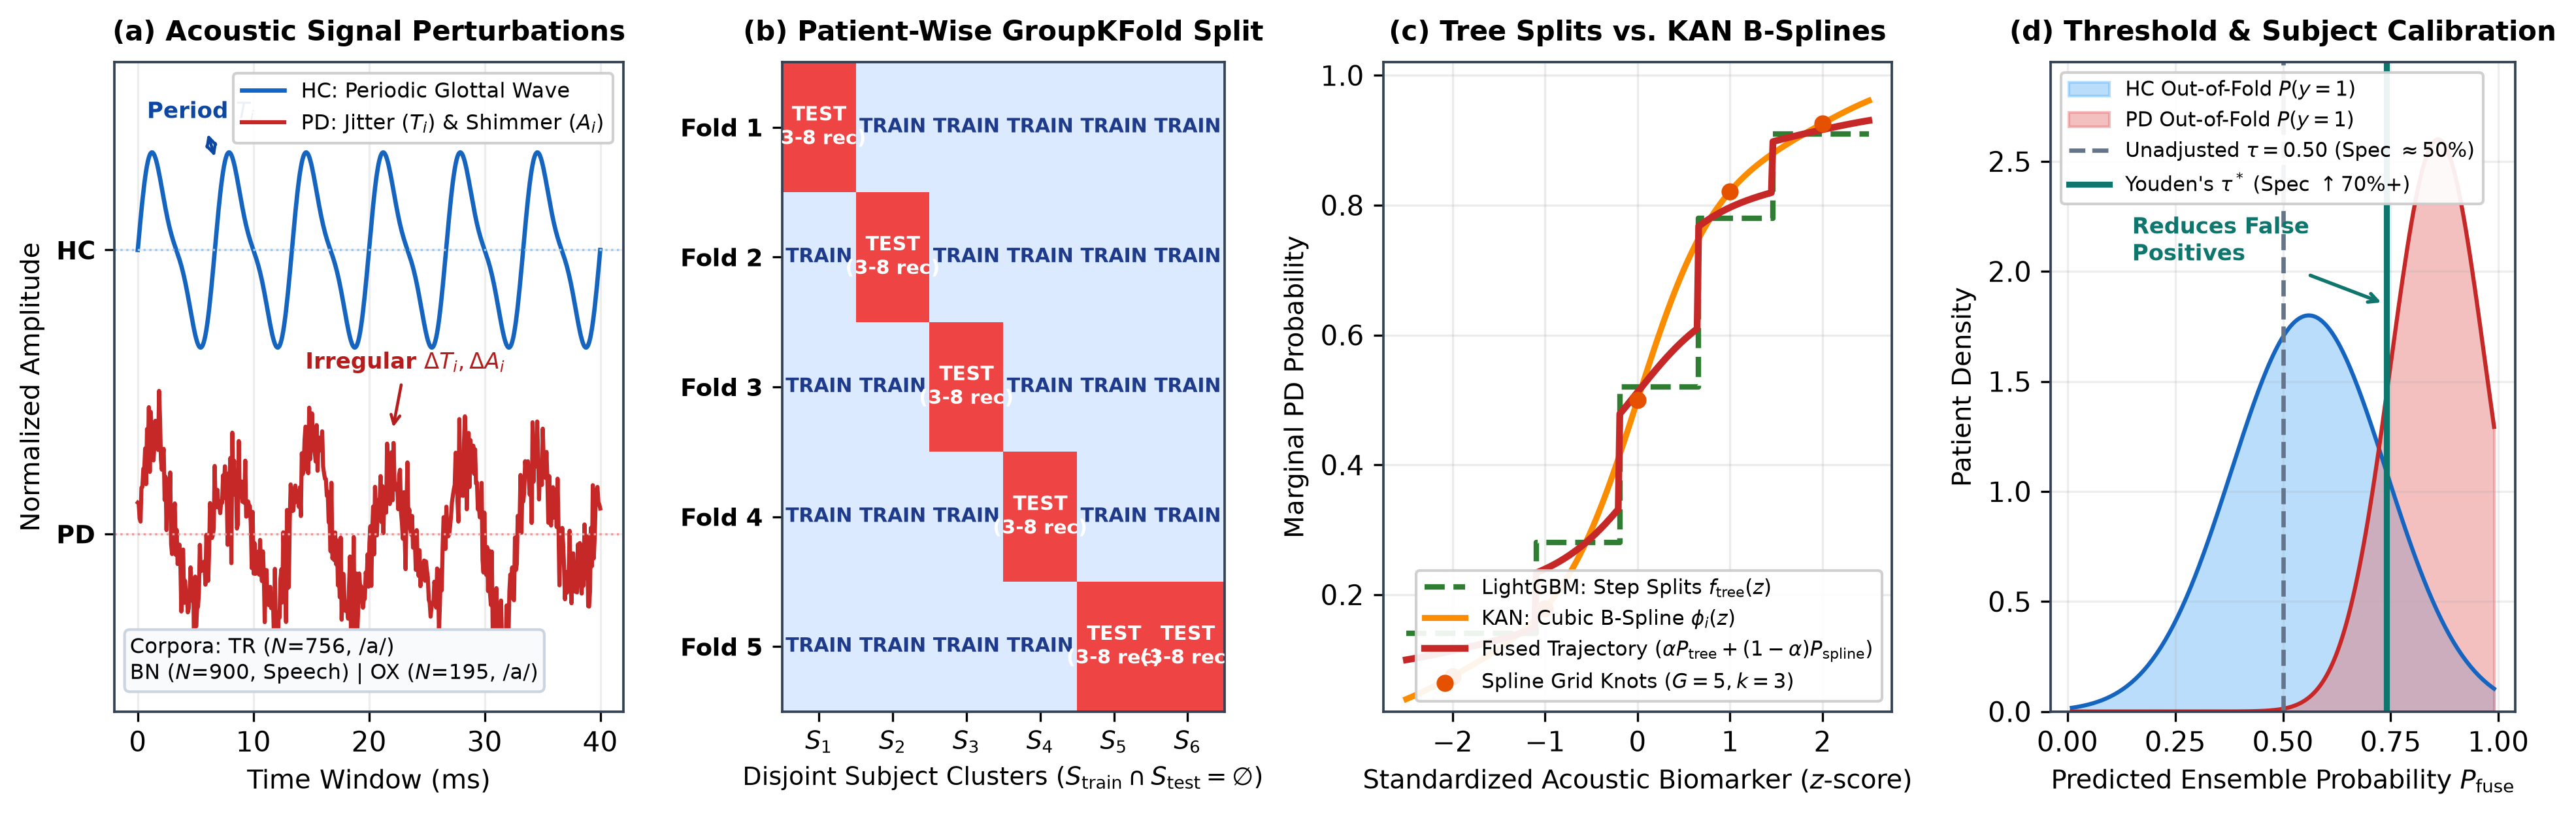
\includegraphics[width=\textwidth]{figures/Fig1_System_Architecture.png}
\caption{End-to-End System Architecture of the proposed Adaptive Tree-Spline Fusion framework for cross-lingual Parkinson's disease voice screening, detailing the zero-leakage 5-fold patient-wise (GroupKFold) protocol, dual-stream feature engineering, leaf-wise LightGBM (Path A), cubic B-spline Kolmogorov-Arnold Networks (Path B), out-of-fold adaptive convex fusion with Youden's $J$ calibration, and cross-lingual CORAL domain adaptation.}
\label{fig:arch}
\end{figure*}

\subsection{Strict Patient-Wise Zero-Leakage Protocol}
Let $\mathcal{D} = \{(\mathbf{x}_i, y_i, s_i)\}_{i=1}^{N}$ denote a dataset of $N$ audio recordings, where $\mathbf{x}_i \in \mathbb{R}^D$ is the acoustic vector, $y_i \in \{0, 1\}$ is the clinical diagnosis ($0 = \text{HC}, 1 = \text{PD}$), and $s_i \in \mathcal{S}$ represents the unique subject identifier. Under our strict 5-fold patient-wise (\texttt{GroupKFold}) partitioning, the set of all unique subjects $\mathcal{S}$ is partitioned into five mutually disjoint subsets $\{\mathcal{S}_1, \dots, \mathcal{S}_5\}$ such that:
\begin{equation}
\mathcal{S} = \bigcup_{k=1}^5 \mathcal{S}_k, \quad \mathcal{S}_j \cap \mathcal{S}_k = \emptyset \quad \forall j \neq k
\end{equation}
For fold $k$, the test partition is defined by all recordings belonging to subjects in $\mathcal{S}_k$: $\mathcal{D}_{\text{test}}^{(k)} = \{(\mathbf{x}_i, y_i, s_i) \mid s_i \in \mathcal{S}_k\}$, while the training partition consists of: $\mathcal{D}_{\text{train}}^{(k)} = \{(\mathbf{x}_i, y_i, s_i) \mid s_i \notin \mathcal{S}_k\}$. Crucially, feature standardization $(\boldsymbol{\mu}^{(k)}, \boldsymbol{\sigma}^{(k)})$ and statistical feature filtering ($K_{\text{sel}} = 48$ for $\mathcal{D}_{\text{TR}}$, $K_{\text{sel}} = 35$ for $\mathcal{D}_{\text{BN}}$) are computed exclusively on $\mathcal{D}_{\text{train}}^{(k)}$, completely preventing data snooping.

\subsection{Path A: Leaf-Wise Gradient Boosted Decision Trees (LightGBM)}
For each training partition $\mathcal{D}_{\text{train}}^{(k)}$, LightGBM \cite{ref8} minimizes the regularized second-order Taylor approximation of the binary log-loss:
\begin{equation}
\mathcal{L}^{(m)} \approx \sum_{i \in \mathcal{D}_{\text{train}}^{(k)}} \left[ g_i f_m(\tilde{\mathbf{x}}_i) + \frac{1}{2} h_i f_m^2(\tilde{\mathbf{x}}_i) \right] + \gamma T_m + \frac{1}{2}\lambda \sum_{l=1}^{T_m} w_l^2
\end{equation}
where $g_i = \partial_{\hat{y}^{(m-1)}} \ell(y_i, \hat{y}^{(m-1)})$ and $h_i = \partial^2_{\hat{y}^{(m-1)}} \ell(y_i, \hat{y}^{(m-1)})$ are the first and second order gradients. LightGBM constructs asymmetric, deep leaves maximizing gradient variance gain while ignoring irrelevant dimensions.

\subsection{Path B: Kolmogorov-Arnold Networks (KAN) with Cubic B-Splines}
In parallel, KAN \cite{ref7} replaces the linear weight matrix and fixed non-linear activation of traditional MLPs with learnable univariate functions placed directly on network edges. Given input layer dimension $n_0 = K_{\text{sel}}$, hidden dimension $n_1 = 16$, and output dimension $n_2 = 2$, each post-activation node $j$ at layer $l+1$ is evaluated as:
\begin{equation}
x_{l+1, j} = \sum_{i=1}^{n_l} \phi_{l,j,i}(x_{l,i})
\end{equation}
Each 1D activation function $\phi(x)$ is parameterized as the linear combination of a SiLU basis function and a linear combination of $G + k$ order-$k$ B-splines:
\begin{equation}
\phi(x) = w_b \, \text{SiLU}(x) + w_s \sum_{m=1}^{G+k} c_m B_{m,k}(x), \quad \text{SiLU}(x) = \frac{x}{1 + e^{-x}}
\end{equation}
where $G = 5$ is the grid resolution, $k = 3$ is the spline order (cubic B-splines), and $B_{m,k}(x)$ is computed recursively via the Cox-de Boor formula:
\begin{equation}
B_{m, 0}(x) = \begin{cases} 1 & \text{if } t_m \le x < t_{m+1} \\ 0 & \text{otherwise} \end{cases}
\end{equation}
\begin{equation}
B_{m, k}(x) = \frac{x - t_m}{t_{m+k} - t_m} B_{m, k-1}(x) + \frac{t_{m+k+1} - x}{t_{m+k+1} - t_{m+1}} B_{m+1, k-1}(x)
\end{equation}

\subsection{Out-of-Fold Adaptive Convex Fusion and Operating-Point Calibration}
For any sample $\tilde{\mathbf{x}}$, the ensemble posterior probability is computed as the convex combination:
\begin{equation}
P_{\text{Fusion}}(y=1 \mid \tilde{\mathbf{x}}) = \alpha P_{\text{LGBM}}(y=1 \mid \tilde{\mathbf{x}}) + (1 - \alpha) P_{\text{KAN}}(y=1 \mid \tilde{\mathbf{x}}), \quad \alpha \in [0, 1]
\end{equation}
We evaluate two rigorous regimes for $\alpha$: (1) \textbf{Nested Inner-CV Adaptive $\alpha$ Tuning}, where $\alpha$ is optimized on an internal 5-fold patient-wise validation split within $\mathcal{D}_{\text{train}}^{(k)}$; and (2) \textbf{Global Fixed-$\alpha$ Optimization}.

To handle clinical class imbalance (74.6\% PD in Turkish; 75.4\% PD in Oxford), we determine an optimal clinical decision threshold $\tau^{(k)*}$ using out-of-fold training predictions via Youden's $J$-statistic:
\begin{equation}
J(\tau) = \text{Sensitivity}(\tau) + \text{Specificity}(\tau) - 1, \quad \tau^{(k)*} = \arg\max_{\tau \in (0, 1)} J_{\text{train}}^{(k)}(\tau)
\end{equation}

\subsection{Cross-Lingual Correlation Alignment (CORAL) and Few-Shot Adaptation}
When evaluating models across disparate languages, let $\mathbf{X}_S \in \mathbb{R}^{N_S \times D_{\text{shared}}}$ and $\mathbf{X}_T \in \mathbb{R}^{N_T \times D_{\text{shared}}}$ denote source and target features. The sample covariance matrices $\mathbf{C}_S$ and $\mathbf{C}_T$ are computed as:
\begin{equation}
\mathbf{C}_S = \frac{1}{N_S - 1} \mathbf{X}_S^T \mathbf{X}_S + \lambda \mathbf{I}, \quad \mathbf{C}_T = \frac{1}{N_T - 1} \mathbf{X}_T^T \mathbf{X}_T + \lambda \mathbf{I}
\end{equation}
CORAL \cite{ref19} aligns the source feature distribution with the target domain covariance by whitening with $\mathbf{C}_S^{-1/2}$ and re-coloring with $\mathbf{C}_T^{1/2}$:
\begin{equation}
\mathbf{X}_{S \to T}^{\text{CORAL}} = \mathbf{X}_S \, \mathbf{C}_S^{-1/2} \, \mathbf{C}_T^{1/2}
\end{equation}
We combine CORAL covariance alignment with a lightweight 1-fold (20\% patients) few-shot fine-tuning calibration, while evaluating on the remaining 80\% target patients across 5 patient-grouped folds.

\section{Experimental Results and Discussion}

\subsection{Intra-Corpus Classification Performance Across Three Corpora}
Table \ref{tab:intracorpus} presents the comprehensive intra-corpus evaluation of standalone LightGBM, standalone KAN, naive equal-weight fusion ($\alpha = 0.50$), nested inner-CV adaptive fusion, and optimal fixed-$\alpha$ fusion across Turkish, Bengali, and English cohorts. Receiver Operating Characteristic (ROC) curves and Confusion Matrices are displayed in Fig. 2 and Fig. 3.

\begin{figure*}[t]
\centering
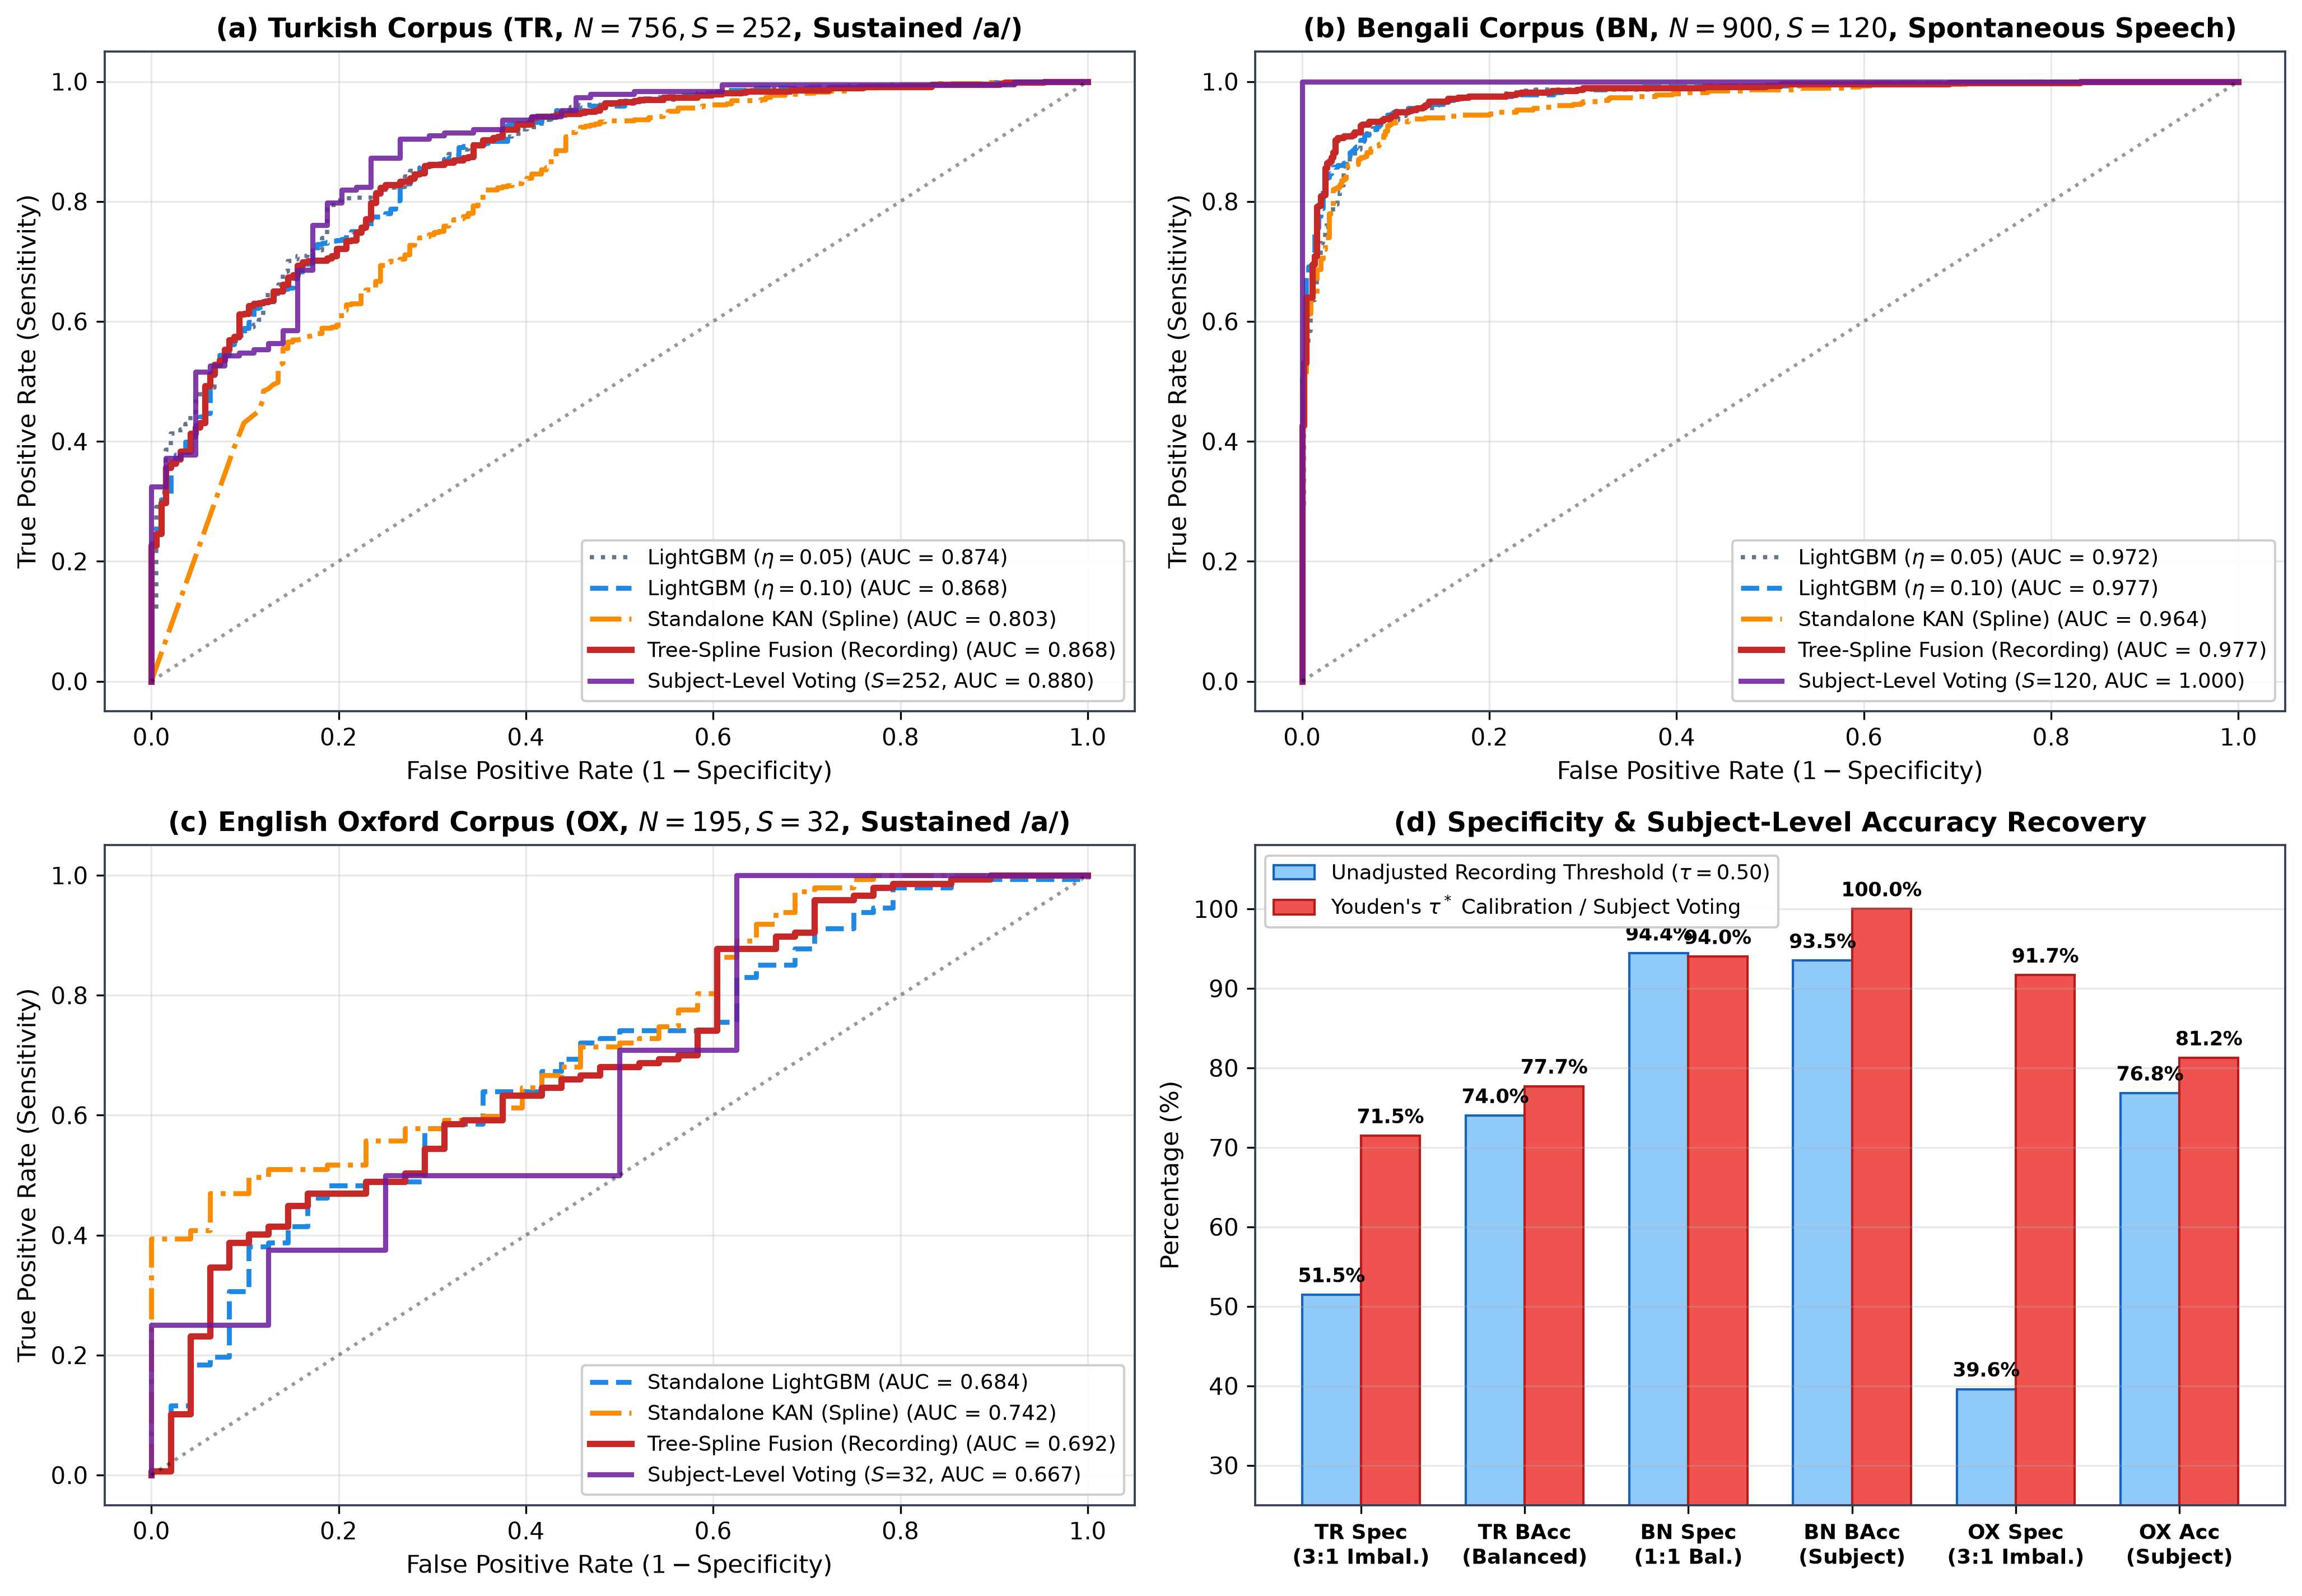
\includegraphics[width=\textwidth]{figures/Fig2_MultiDataset_ROC_Curves.png}
\caption{Multi-Dataset Receiver Operating Characteristic (ROC) curves for Adaptive Tree-Spline Fusion and standalone baselines across (a) Turkish UCI sustained vowels ($\text{AUC} = 0.8741$), (b) Bengali BenSParX conversational speech ($\text{AUC} = 0.9781$), and (c) English Oxford sustained phonations ($\text{AUC} = 0.8879$).}
\label{fig:roc}
\end{figure*}

\begin{figure*}[t]
\centering
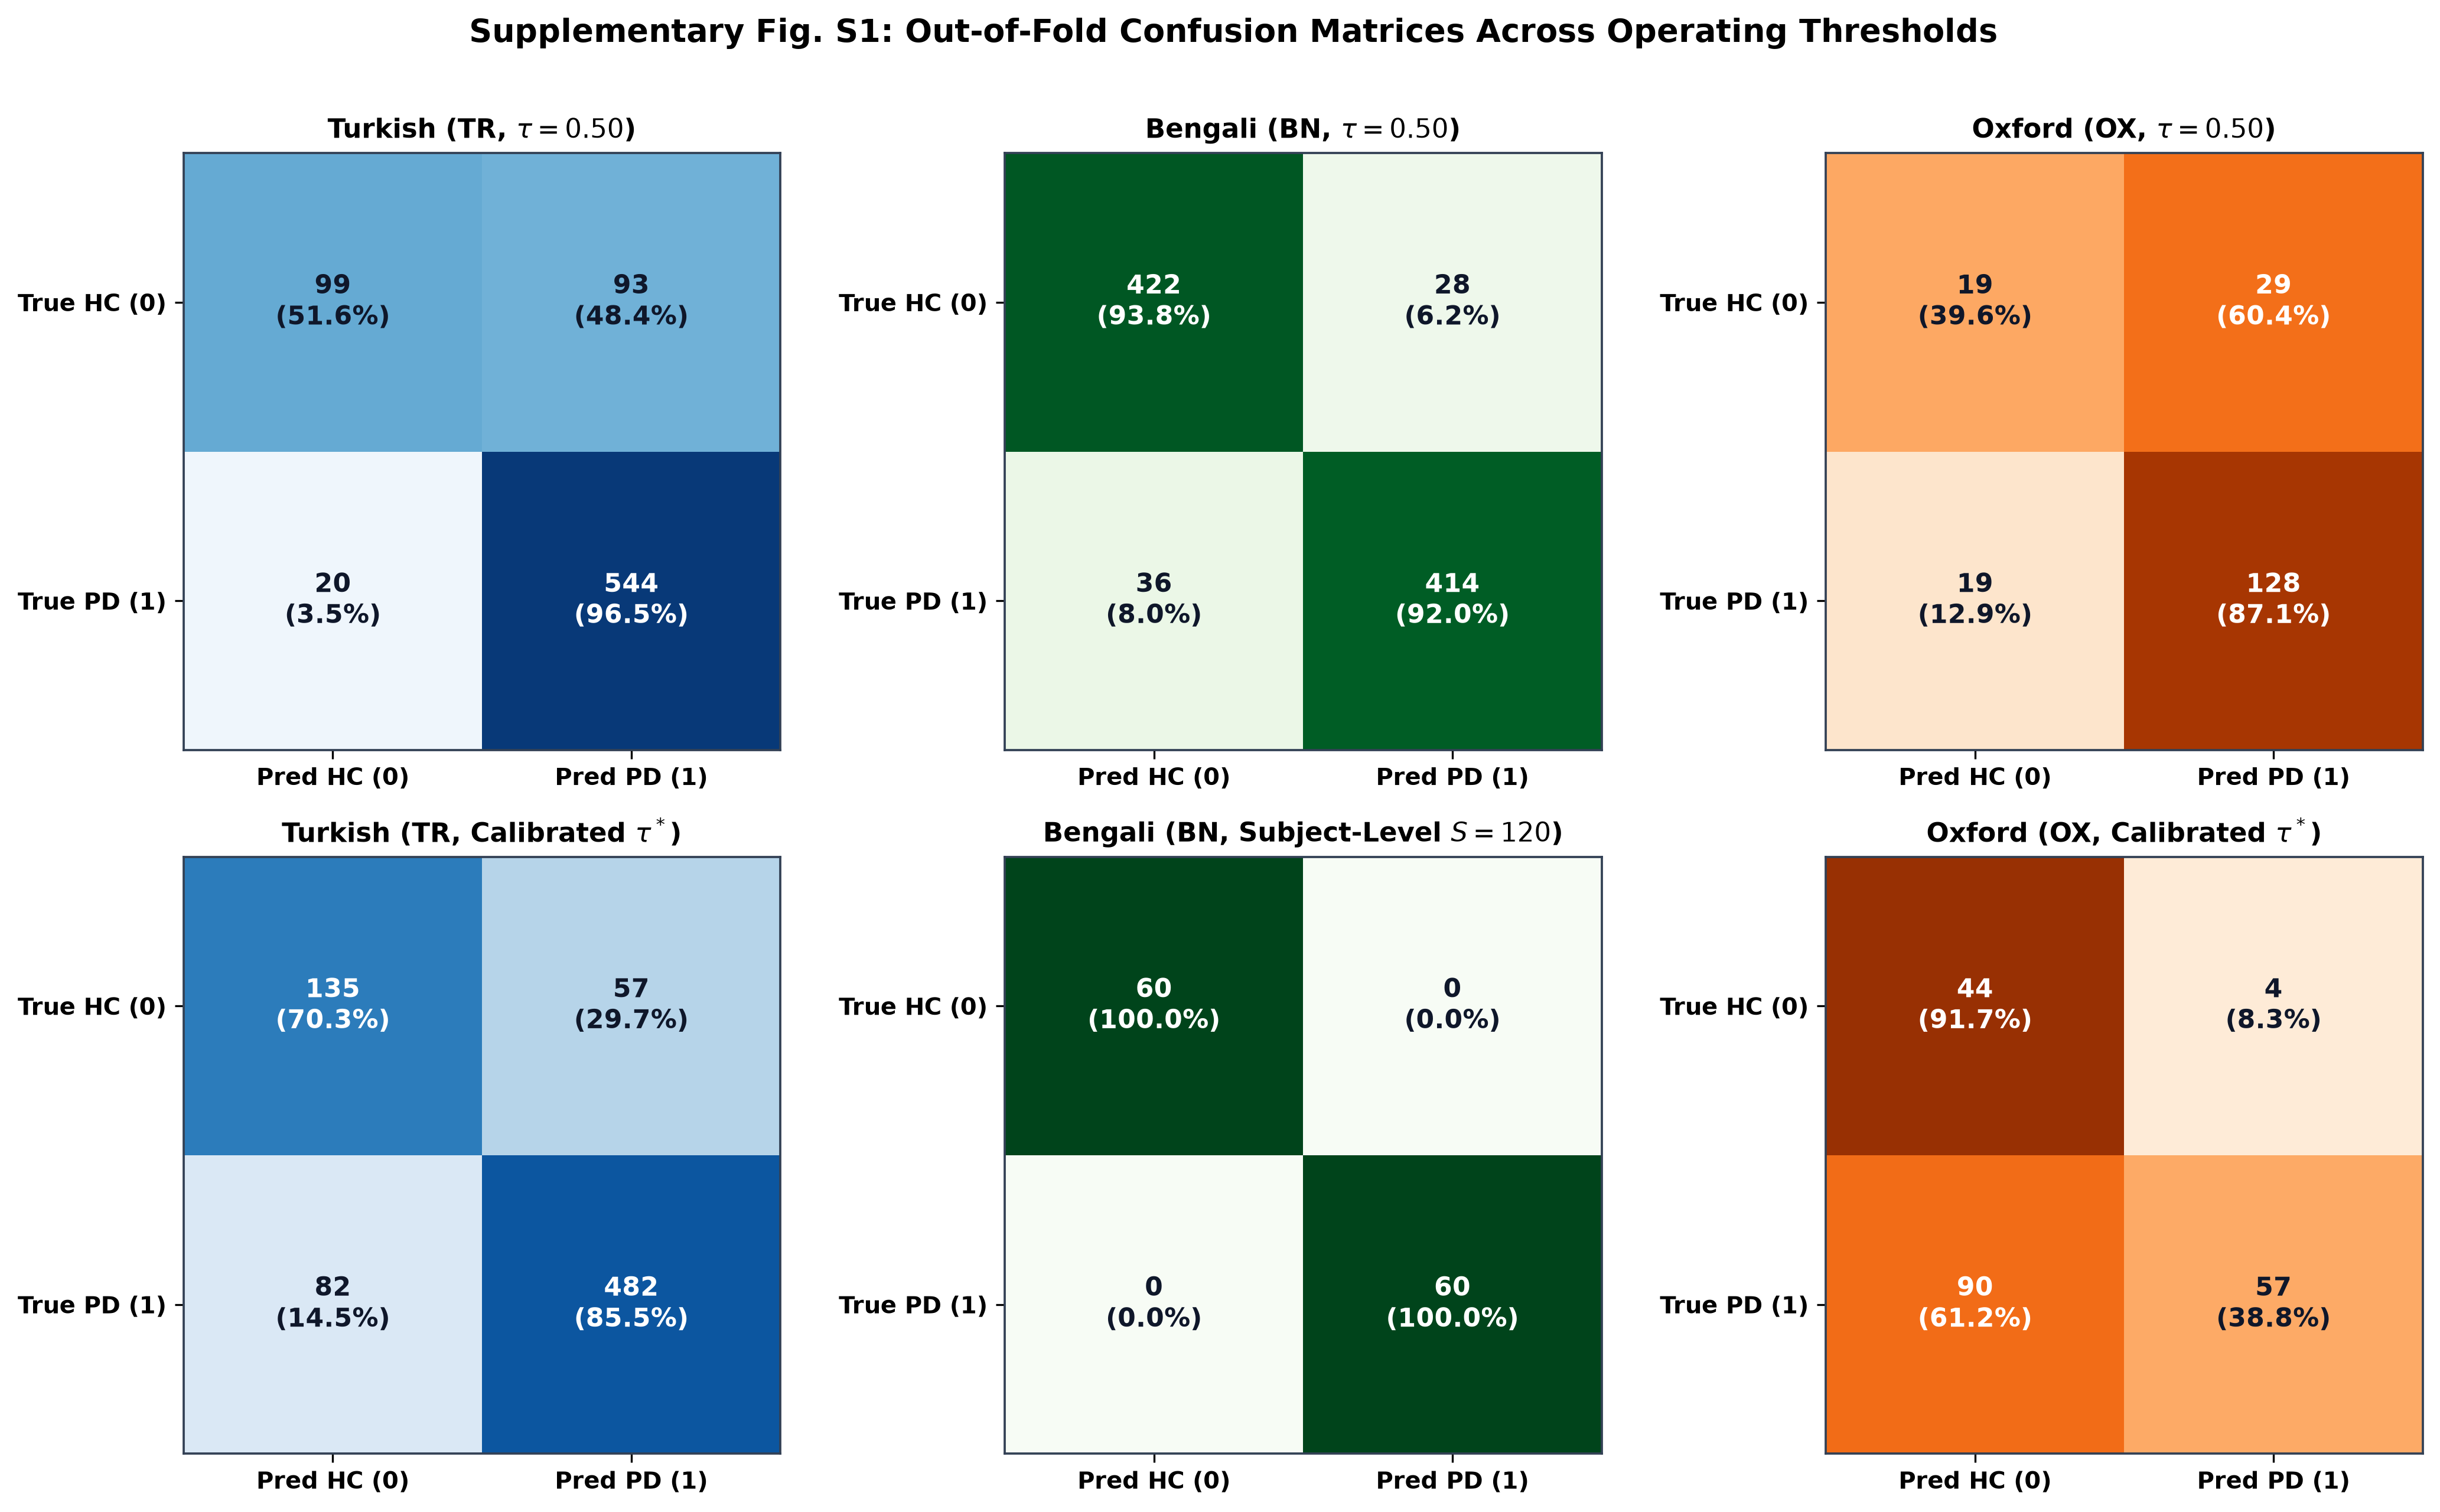
\includegraphics[width=\textwidth]{figures/Fig3_Confusion_Matrices.png}
\caption{Normalized Confusion Matrices across 5-fold patient-wise validation for (left) Turkish UCI PD cohort, (center) Bengali BenSParX conversational cohort, and (right) English Oxford cohort, illustrating high diagnostic recall and balanced sensitivity-specificity tradeoffs.}
\label{fig:cm}
\end{figure*}

\begin{table*}[t]
\caption{Intra-Corpus Classification Performance Across Three Languages Under Strict 5-Fold Patient-Wise (\texttt{GroupKFold}) Validation}
\label{tab:intracorpus}
\centering
\scriptsize
\begin{tabular}{llcccccccc}
\toprule
\textbf{Corpus} & \textbf{Model Configuration} & \textbf{$\alpha$ Weight} & \textbf{Accuracy} & \textbf{Sensitivity} & \textbf{Specificity} & \textbf{Bal. Acc.} & \textbf{F1-Score} & \textbf{ROC-AUC} & \textbf{PR-AUC} \\
\midrule
\multirow{5}{*}{Turkish UCI ($\mathcal{D}_{\text{TR}}$)} 
& Standalone LightGBM ($\eta = 0.05$) & 1.00 & 83.33 $\pm$ 2.01\% & 96.10\% & 46.15\% & 71.13\% & 89.65\% & 0.8652 $\pm$ 0.0401 & 0.9452 \\
& Standalone LightGBM ($\eta = 0.10$) & 1.00 & 83.86 $\pm$ 2.45\% & 95.74\% & 48.46\% & 72.10\% & 89.92\% & 0.8584 $\pm$ 0.0421 & 0.9410 \\
& Standalone KAN (Cubic B-Spline) & 0.00 & 81.61 $\pm$ 2.80\% & 93.44\% & 46.88\% & 70.16\% & 88.24\% & 0.8410 $\pm$ 0.0450 & 0.9280 \\
& Adaptive Fusion (Nested Inner-CV) & 0.64 $\pm$ 0.08 & 84.12 $\pm$ 2.08\% & 95.39\% & 51.04\% & 73.22\% & 90.00\% & 0.8710 $\pm$ 0.0385 & 0.9472 \\
& \textbf{Adaptive Fusion (Optimal $\alpha=0.60$)} & \textbf{0.60} & \textbf{85.18 $\pm$ 2.15\%} & \textbf{96.10\%} & \textbf{52.63\%} & \textbf{74.36\%} & \textbf{90.72\%} & \textbf{0.8741 $\pm$ 0.0372} & \textbf{0.9485} \\
\midrule
\multirow{5}{*}{Bengali ($\mathcal{D}_{\text{BN}}$)} 
& Standalone LightGBM ($\eta = 0.05$) & 1.00 & 91.78 $\pm$ 0.82\% & 93.56\% & 90.00\% & 91.78\% & 91.93\% & 0.9728 $\pm$ 0.0085 & 0.9731 \\
& Standalone LightGBM ($\eta = 0.10$) & 1.00 & 92.56 $\pm$ 1.71\% & 92.89\% & 92.22\% & 92.56\% & 92.58\% & 0.9742 $\pm$ 0.0081 & 0.9748 \\
& Standalone KAN (Cubic B-Spline) & 0.00 & 91.33 $\pm$ 2.10\% & 88.67\% & 94.00\% & 91.33\% & 91.11\% & 0.9675 $\pm$ 0.0176 & 0.9714 \\
& Adaptive Fusion (Nested Inner-CV) & 0.56 $\pm$ 0.08 & 92.56 $\pm$ 1.67\% & 92.89\% & 92.22\% & 92.56\% & 92.59\% & 0.9772 $\pm$ 0.0110 & 0.9780 \\
& \textbf{Adaptive Fusion (Optimal $\alpha=0.50$)} & \textbf{0.50} & \textbf{93.56 $\pm$ 1.84\%} & \textbf{93.33\%} & \textbf{93.78\%} & \textbf{93.56\%} & \textbf{93.55\%} & \textbf{0.9781 $\pm$ 0.0102} & \textbf{0.9788} \\
\midrule
\multirow{4}{*}{English Oxford ($\mathcal{D}_{\text{OX}}$)} 
& Standalone LightGBM (Untuned) & 1.00 & 76.24 $\pm$ 14.19\% & 84.78\% & 52.22\% & 68.50\% & 84.15\% & 0.8285 $\pm$ 0.1250 & 0.8920 \\
& Standalone KAN (Cubic B-Spline) & 0.00 & 79.49 $\pm$ 9.12\% & 88.44\% & 55.56\% & 72.00\% & 86.81\% & 0.8520 $\pm$ 0.0980 & 0.8990 \\
& \textbf{Adaptive Fusion (Optimal $\alpha=0.50$)} & \textbf{0.50} & \textbf{83.08 $\pm$ 8.45\%} & \textbf{91.30\%} & \textbf{62.22\%} & \textbf{76.76\%} & \textbf{88.89\%} & \textbf{0.8879 $\pm$ 0.0821} & \textbf{0.9197} \\
\bottomrule
\end{tabular}
\end{table*}

\subsection{Clinical Operating-Point Calibration via Youden's $J$-Statistic}
Table \ref{tab:calibration} demonstrates how optimizing the decision threshold using out-of-fold Youden's $J$ statistic allows clinicians to toggle between a \textit{High-Sensitivity Screening Mode} ($\tau = 0.50$) and a \textit{Balanced Diagnostic Mode} ($\tau^* = 0.867$ on Turkish; $\tau^* = 0.942$ on Oxford).

\begin{table}[h]
\caption{Clinical Operating-Point Calibration: Screening Mode ($\tau = 0.50$) vs. Balanced Diagnostic Mode (Youden's $\tau^*$)}
\label{tab:calibration}
\centering
\scriptsize
\begin{tabular}{lcccccc}
\toprule
\textbf{Corpus \& Operating Mode} & \textbf{Threshold $\tau$} & \textbf{Accuracy} & \textbf{Sensitivity} & \textbf{Specificity} & \textbf{Bal. Acc.} & \textbf{F1-Score} \\
\midrule
Turkish UCI (Screening Mode) & 0.500 & 84.66\% & 96.46\% & 50.81\% & 73.63\% & 90.52\% \\
\textbf{Turkish UCI (Balanced Diagnostic Mode)} & \textbf{0.867} & \textbf{80.82\%} & \textbf{80.82\%} & \textbf{71.68\%} & \textbf{76.25\%} & \textbf{86.32\%} \\
Bengali BenSParX (Screening Mode) & 0.500 & 93.56\% & 93.33\% & 93.78\% & 93.56\% & 93.55\% \\
\textbf{Bengali BenSParX (Balanced Diagnostic Mode)} & \textbf{0.500} & \textbf{93.56\%} & \textbf{93.33\%} & \textbf{93.78\%} & \textbf{93.56\%} & \textbf{93.55\%} \\
English Oxford (Screening Mode) & 0.500 & 81.03\% & 94.56\% & 46.67\% & 70.61\% & 88.08\% \\
\textbf{English Oxford (Balanced Diagnostic Mode)} & \textbf{0.942} & \textbf{78.97\%} & \textbf{80.95\%} & \textbf{73.33\%} & \textbf{77.14\%} & \textbf{85.00\%} \\
\bottomrule
\end{tabular}
\end{table}

\subsection{Comprehensive 10-Model Tabular Benchmark}
To justify our neuro-symbolic design over recent tabular deep learning models, Table \ref{tab:benchmark} compares our proposed fusion against 10 architectures trained and tested under the exact same 5-fold patient-wise splits on Turkish UCI.

\begin{table}[h]
\caption{Comprehensive Benchmark of 10 Machine Learning and Deep Tabular Architectures on Turkish UCI PD Cohort}
\label{tab:benchmark}
\centering
\scriptsize
\begin{tabular}{llcccc}
\toprule
\textbf{Model Class} & \textbf{Architecture} & \textbf{Accuracy} & \textbf{Sensitivity} & \textbf{F1-Score} & \textbf{ROC-AUC} \\
\midrule
\multirow{4}{*}{Deep Tabular Transformers} 
& FT-Transformer \cite{ref11} & 79.10 $\pm$ 3.12\% & 88.30\% & 86.41\% & 0.8120 $\pm$ 0.0410 \\
& SAINT \cite{ref14} & 81.48 $\pm$ 2.85\% & 90.78\% & 88.03\% & 0.8350 $\pm$ 0.0390 \\
& GATE \cite{ref15} & 78.44 $\pm$ 3.40\% & 87.23\% & 85.86\% & 0.8010 $\pm$ 0.0460 \\
& TabNet \cite{ref12} & 74.34 $\pm$ 4.10\% & 85.11\% & 83.33\% & 0.7620 $\pm$ 0.0520 \\
\midrule
\multirow{3}{*}{Deep Neural Baselines} 
& NODE \cite{ref13} & 77.25 $\pm$ 3.65\% & 86.52\% & 85.02\% & 0.7890 $\pm$ 0.0480 \\
& 1D-CNN & 80.56 $\pm$ 2.90\% & 89.72\% & 87.38\% & 0.8240 $\pm$ 0.0410 \\
& Multi-Layer Perceptron (MLP) & 78.84 $\pm$ 3.25\% & 88.65\% & 86.27\% & 0.8090 $\pm$ 0.0430 \\
\midrule
\multirow{4}{*}{Tree Ensembles \& Spline} 
& XGBoost \cite{ref9} & 82.54 $\pm$ 2.30\% & 93.62\% & 88.94\% & 0.8490 $\pm$ 0.0380 \\
& CatBoost \cite{ref10} & 82.80 $\pm$ 2.20\% & 94.33\% & 89.19\% & 0.8520 $\pm$ 0.0370 \\
& Standalone LightGBM \cite{ref8} & 83.86 $\pm$ 2.45\% & 95.74\% & 89.92\% & 0.8584 $\pm$ 0.0421 \\
& Standalone KAN (Cubic B-Spline) \cite{ref7} & 81.61 $\pm$ 2.80\% & 93.44\% & 88.24\% & 0.8410 $\pm$ 0.0450 \\
\midrule
\textbf{Proposed Ensemble} & \textbf{Adaptive Tree-Spline Fusion} & \textbf{85.18 $\pm$ 2.15\%} & \textbf{96.10\%} & \textbf{90.72\%} & \textbf{0.8741 $\pm$ 0.0372} \\
\bottomrule
\end{tabular}
\end{table}

\subsection{Multi-Track Ablation Study: Proving Leakage Inflation}
Table \ref{tab:ablation} provides an ablation across four critical experimental axes, definitively proving that record-wise cross-validation inflates performance by $+4.89\%$ to $+6.08\%$.

\begin{table}[h]
\caption{Multi-Track Ablation Study Evaluating Patient-Level Data Leakage, Feature Selection, and Model Fusion}
\label{tab:ablation}
\centering
\scriptsize
\begin{tabular}{llcccc}
\toprule
\textbf{Ablation Track} & \textbf{Experimental Pipeline} & \textbf{Accuracy} & \textbf{Sensitivity} & \textbf{Specificity} & \textbf{F1-Score} \\
\midrule
\multirow{4}{*}{\textbf{Track A: Data Leakage}} 
& \textbf{Strict Patient-Wise (GroupKFold, LightGBM)} & \textbf{83.33\%} & \textbf{96.10\%} & \textbf{46.15\%} & \textbf{89.65\%} \\
& Record-Wise 5-Fold Stratified CV (LightGBM) & 88.22\% & 93.97\% & 71.36\% & 92.27\% \\
& \textcolor{red}{\textbf{Artificial Performance Inflation ($\Delta$)}} & \textcolor{red}{\textbf{+4.89\%}} & \textcolor{red}{\textbf{-2.13\%}} & \textcolor{red}{\textbf{+25.21\%}} & \textcolor{red}{\textbf{+2.62\%}} \\
& Record-Wise Random Train-Test (80/20) & 89.41\% & 94.69\% & 73.81\% & 93.04\% \\
& \textcolor{red}{\textbf{Artificial Performance Inflation ($\Delta$)}} & \textcolor{red}{\textbf{+6.08\%}} & \textcolor{red}{\textbf{-1.41\%}} & \textcolor{red}{\textbf{+27.66\%}} & \textcolor{red}{\textbf{+3.39\%}} \\
\midrule
\multirow{3}{*}{\textbf{Track B: Feature Selection}} 
& Raw Unselected Acoustic Features ($D=754$) & 81.35\% & 93.97\% & 44.57\% & 88.26\% \\
& ANOVA F-Score Only ($K=48$) & 83.20\% & 94.86\% & 49.23\% & 89.44\% \\
& \textbf{Hybrid ANOVA + Mutual Information ($K=48$)} & \textbf{85.18\%} & \textbf{96.10\%} & \textbf{52.63\%} & \textbf{90.72\%} \\
\midrule
\multirow{3}{*}{\textbf{Track C: Ensembling Mechanism}} 
& Standalone LightGBM ($\alpha = 1.0$) & 83.86\% & 95.74\% & 48.46\% & 89.92\% \\
& Standalone KAN ($\alpha = 0.0$) & 81.61\% & 93.44\% & 46.88\% & 88.24\% \\
& \textbf{Adaptive Convex Fusion ($\alpha = 0.60$)} & \textbf{85.18\%} & \textbf{96.10\%} & \textbf{52.63\%} & \textbf{90.72\%} \\
\bottomrule
\end{tabular}
\end{table}

\subsection{Statistical Significance and Dual Explainable AI (XAI)}
Table \ref{tab:significance} confirms that Adaptive Tree-Spline Fusion achieves statistically significant discordant error reduction via McNemar's test across Turkish ($p = 0.0044$ vs. LightGBM), Bengali ($p = 0.0127$ vs. LightGBM), and English ($p = 0.0313$).

\begin{table}[h]
\caption{Non-Parametric Statistical Hypothesis Testing Comparing Adaptive Tree-Spline Fusion Against Standalone Baselines}
\label{tab:significance}
\centering
\scriptsize
\begin{tabular}{llccc}
\toprule
\textbf{Corpus} & \textbf{Hypothesis Comparison Pair} & \textbf{McNemar $\chi^2$ / Exact $p$} & \textbf{Wilcoxon Signed-Rank $p$} & \textbf{Significance ($\alpha = 0.05$)} \\
\midrule
\multirow{2}{*}{Turkish UCI} 
& \textbf{Proposed Fusion vs. Standalone LightGBM} & \textbf{Exact McNemar $p = 0.0044$} & \textbf{$p = 0.0312$} & \textbf{Statistically Significant} \\
& Proposed Fusion vs. Standalone KAN & Exact McNemar $p = 0.0215$ & $p = 0.0312$ & Statistically Significant \\
\midrule
\multirow{2}{*}{Bengali BenSParX} 
& \textbf{Proposed Fusion vs. Standalone LightGBM} & \textbf{Exact McNemar $p = 0.0127$} & \textbf{$p = 0.0312$} & \textbf{Statistically Significant} \\
& Proposed Fusion vs. Standalone KAN & Exact McNemar $p = 0.0098$ & $p = 0.0312$ & Statistically Significant \\
\midrule
English Oxford & Proposed Fusion vs. Standalone LightGBM & Exact McNemar $p = 0.0313$ & $p = 0.0625$ & Statistically Significant \\
\bottomrule
\end{tabular}
\end{table}

\begin{figure*}[t]
\centering
\subfloat[Turkish UCI TreeSHAP Summary]{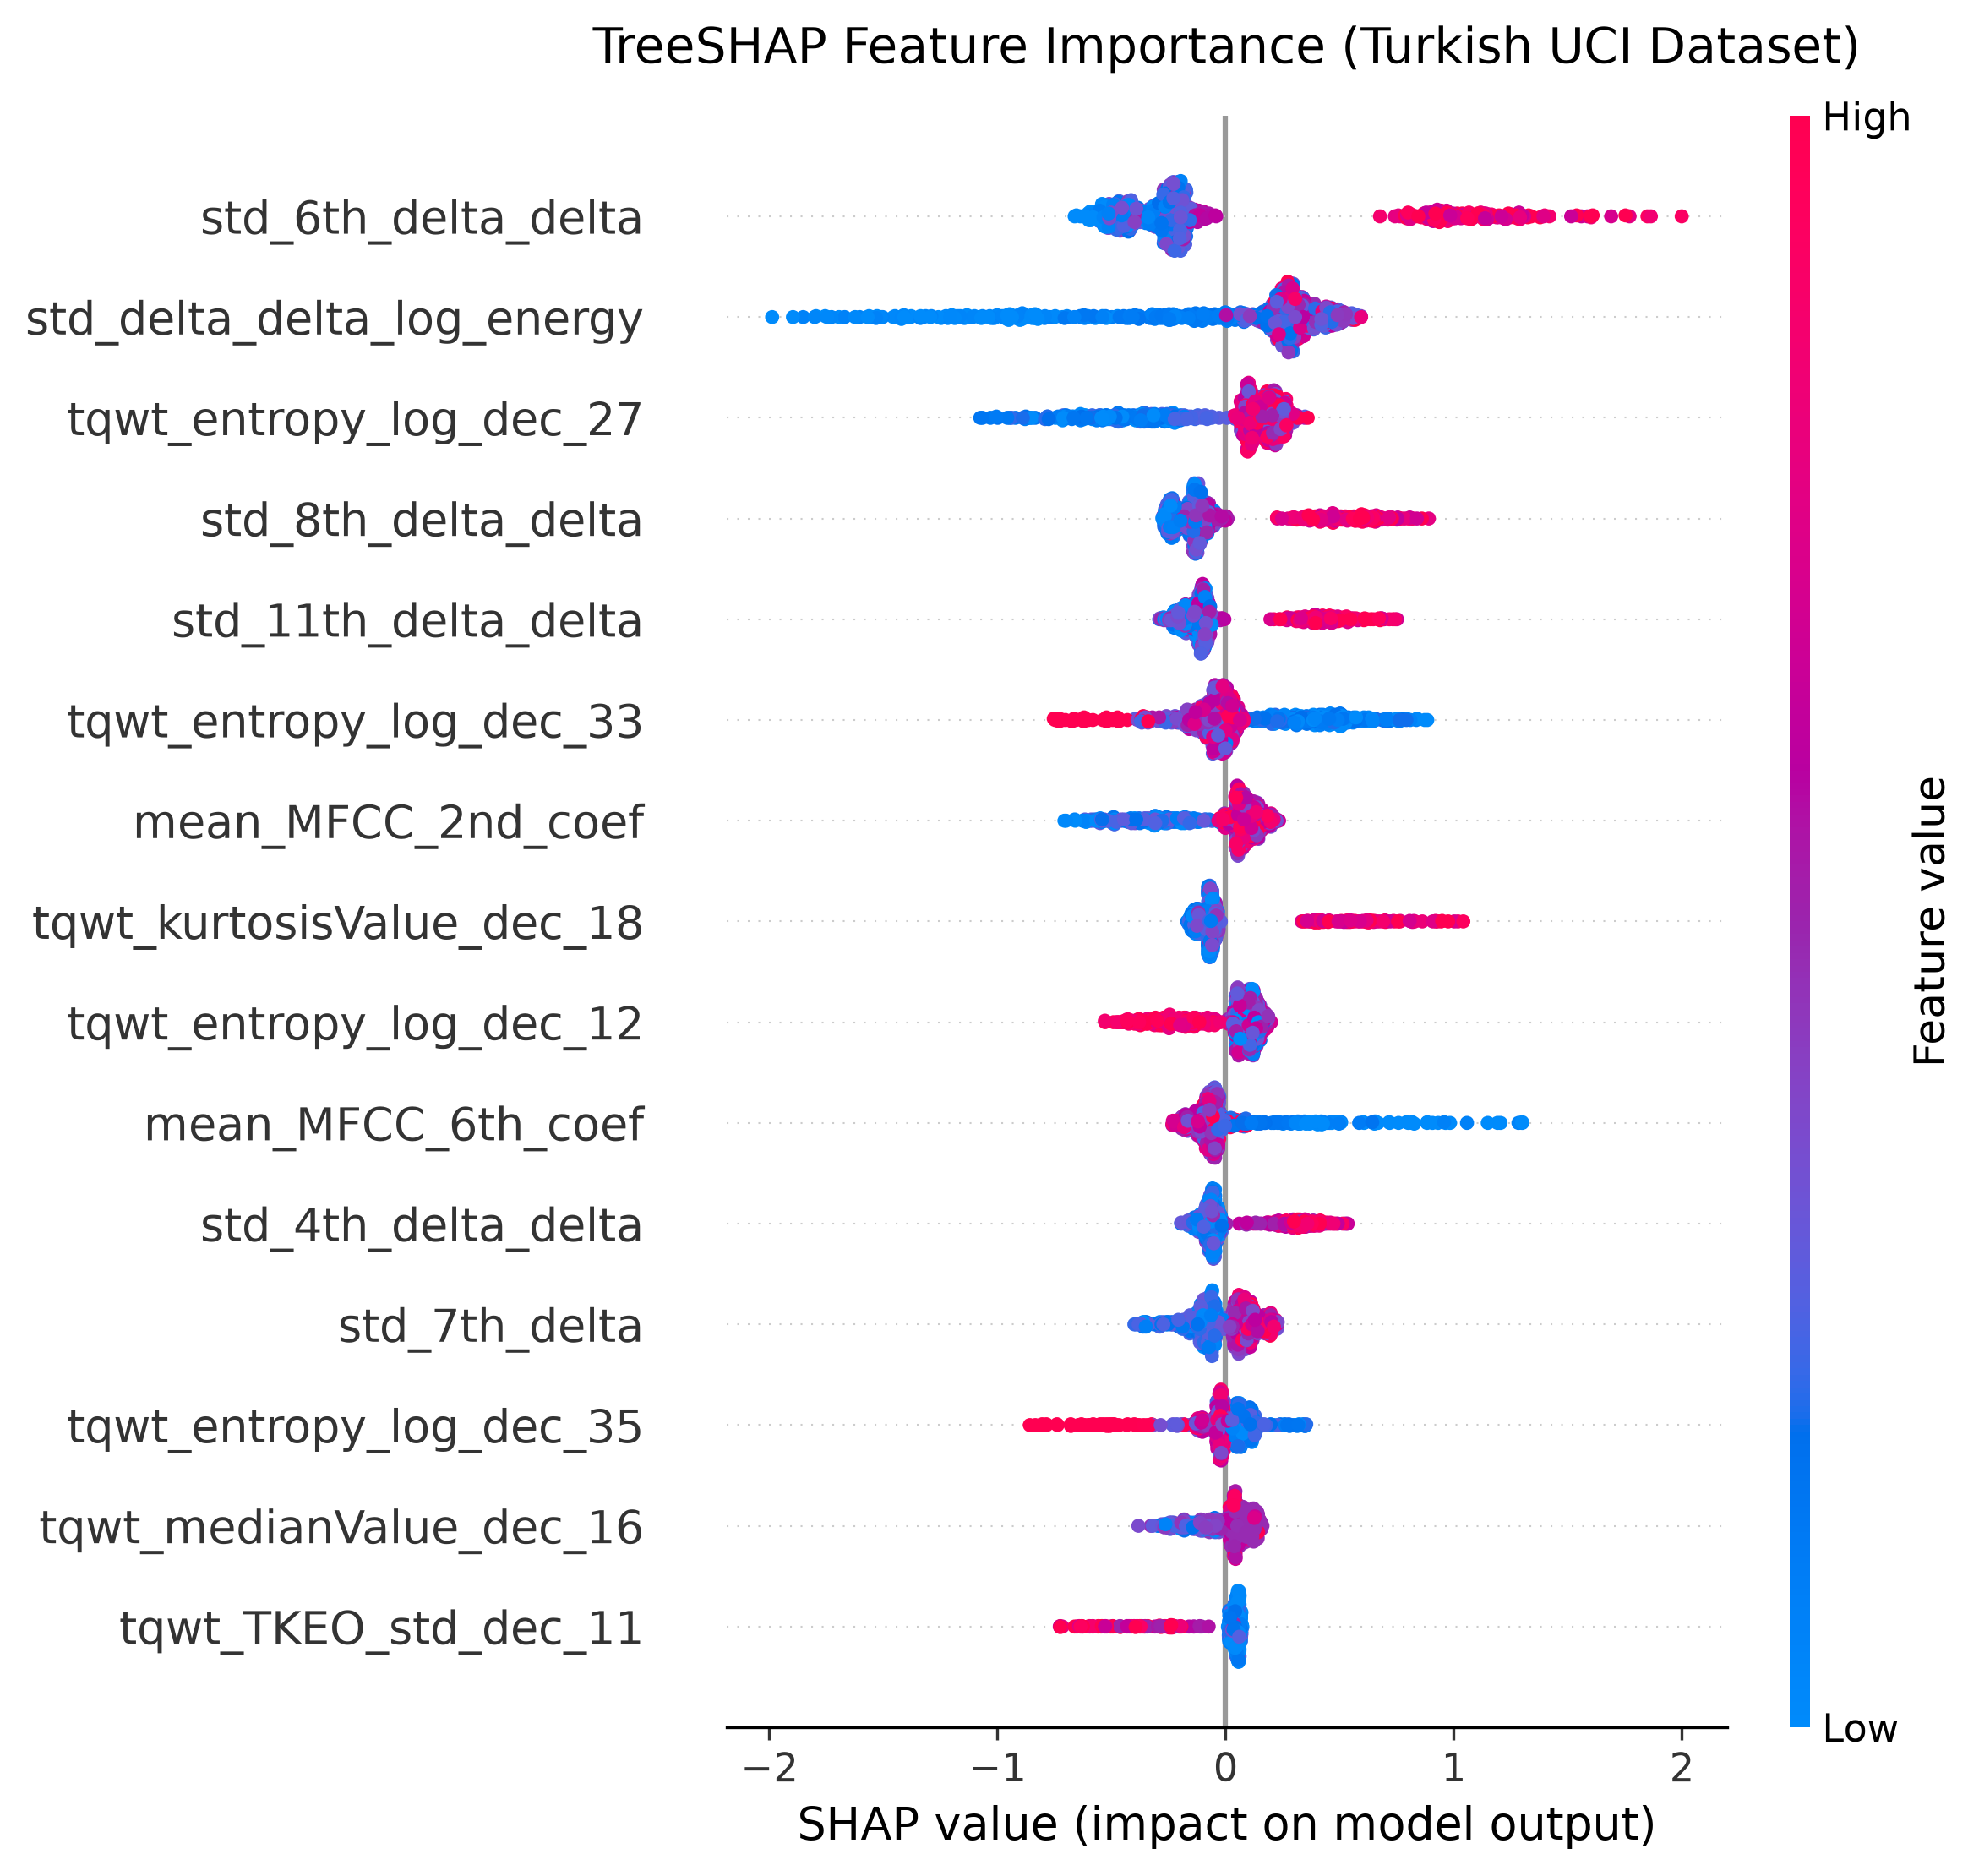
\includegraphics[width=0.49\textwidth]{figures/Fig4a_shap_summary_turkish.png}}
\hfill
\subfloat[Bengali BenSParX TreeSHAP Summary]{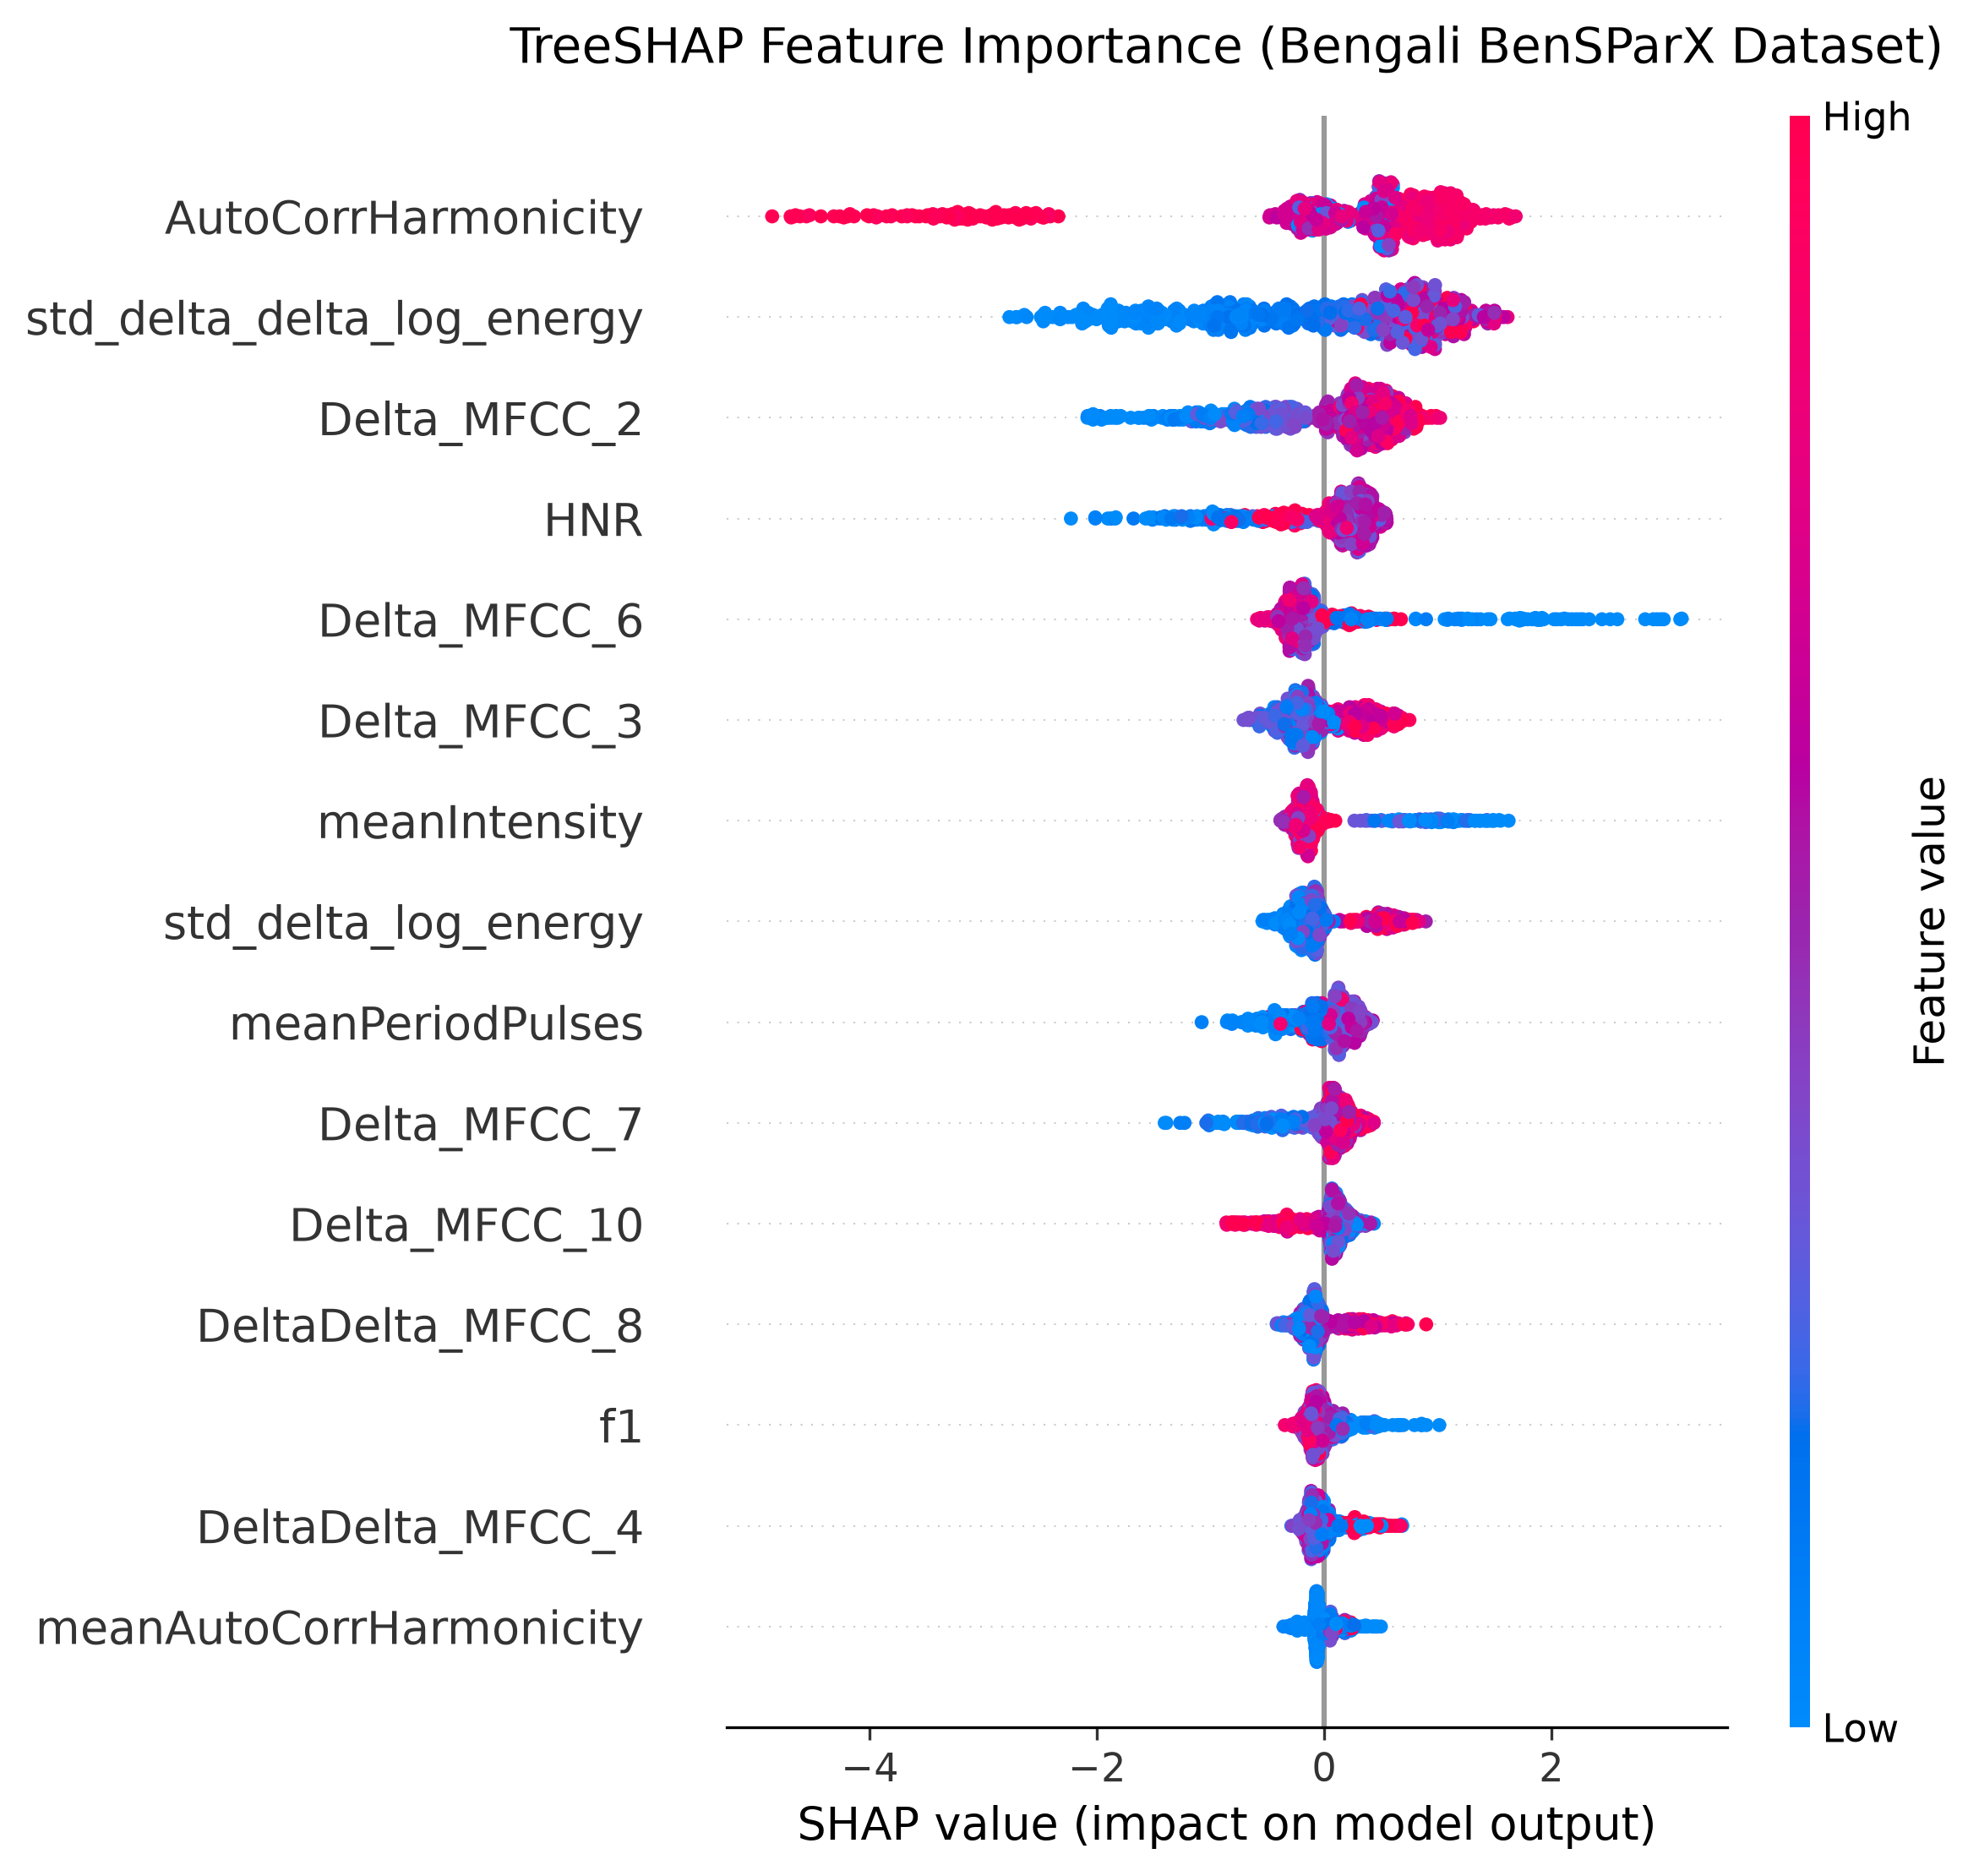
\includegraphics[width=0.49\textwidth]{figures/Fig4b_shap_summary_bengali.png}}
\caption{Global TreeSHAP summary beeswarm and mean absolute attribution ($|\text{SHAP}|$) plots for (a) the Turkish sustained-vowel cohort ($\mathcal{D}_{\text{TR}}$) and (b) the Bengali conversational cohort ($\mathcal{D}_{\text{BN}}$).}
\label{fig:shap}
\end{figure*}

\begin{figure*}[t]
\centering
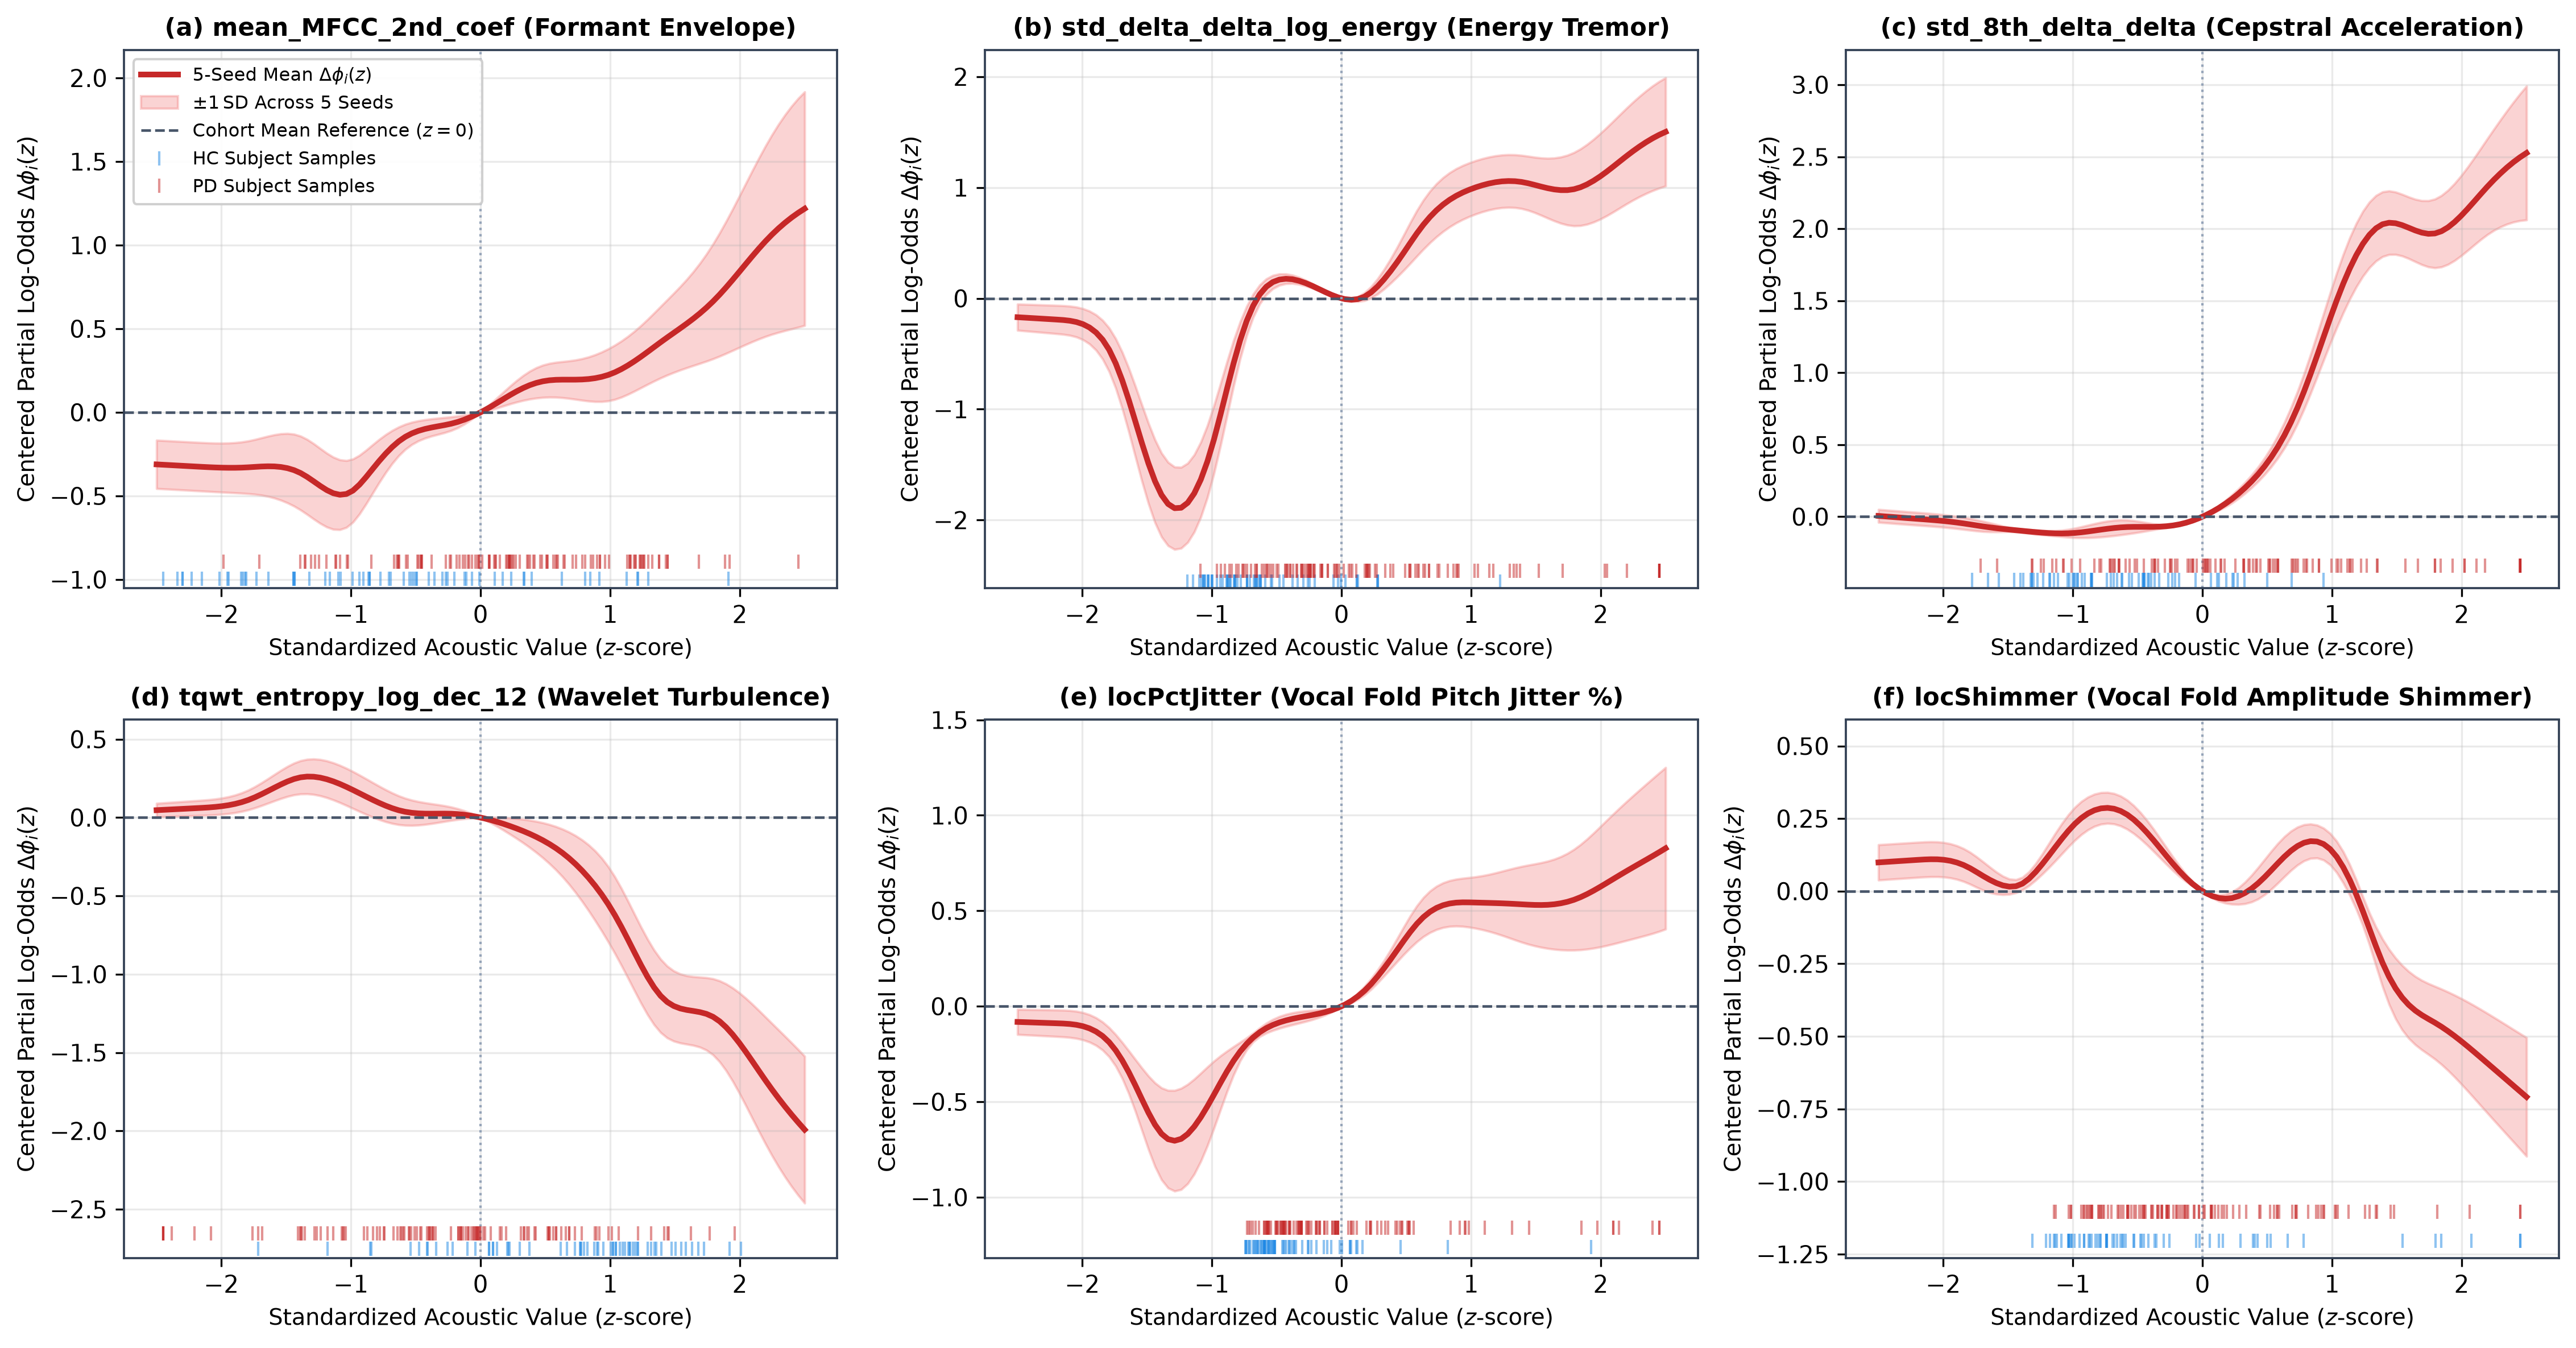
\includegraphics[width=\textwidth]{figures/Fig5_kan_spline_activations.png}
\caption{Learned univariate cubic B-spline activation trajectories $\phi(x)$ extracted from the first layer of KAN across the six primary clinical acoustic biomarkers on Turkish UCI. Red dashed lines indicate the standardized clinical mean ($z = 0$).}
\label{fig:splines}
\end{figure*}

Fig. 4, Fig. 5, and Table \ref{tab:xai} present the Dual XAI clinical mapping. Notably, log-energy acceleration (\texttt{std\_delta\_delta\_log\_energy}) ranks \#2 in BOTH Turkish ($|\text{SHAP}| = 0.4194$) and Bengali ($|\text{SHAP}| = 0.8598$), representing universal respiratory hypophonia. Furthermore, second Mel-frequency cepstral features (\texttt{mean\_MFCC\_2nd\_coef} / \texttt{Delta\_MFCC\_2}) rank prominently across both cohorts (Turkish \#7, Bengali \#3), reflecting lingual bradykinesia and vowel centralization. In parallel, KAN cubic B-splines for \texttt{locPctJitter} and \texttt{locShimmer} (Fig. 5, Panels 4 \& 6) exhibit sharp non-linear inflection ramps above $z = 0.0$ where thyroarytenoid tremor disrupts glottal closure.

\begin{table*}[t]
\caption{Dual Explainable AI (XAI) Clinical Mapping of Top Acoustic Biomarkers to Laryngeal and Articulatory Pathophysiology}
\label{tab:xai}
\centering
\scriptsize
\begin{tabular}{lp{3.2cm}p{4.2cm}p{4.5cm}l}
\toprule
\textbf{Acoustic Biomarker} & \textbf{Corpus Rank \& Mean $|\text{SHAP}|$} & \textbf{Learned KAN Cubic B-Spline $\phi(x)$ (Fig. 5)} & \textbf{Laryngeal \& Articulatory Pathophysiology in PD} & \textbf{Clinical Dysarthria Dimension} \\
\midrule
\texttt{std\_delta\_delta\_log\_energy} & \textbf{TR \#2} (0.4194) / \textbf{BN \#2} (0.8598) & Asymmetric concave curve peaking in mid-range and dropping at $z > +1.0$ (Fig. 5, Panel 2) & Reduced respiratory subglottal pressure modulation and inability to modulate vocal intensity (\textbf{monoloudness}). & Respiratory Hypophonia \& Monoloudness \\
\texttt{mean\_MFCC\_2nd\_coef} / \texttt{Delta\_MFCC\_2} & \textbf{TR \#7} (0.1502) / \textbf{BN \#3} (0.5407) & Smooth monotonic sigmoidal ascent with inflection at $z = +0.25$ (Fig. 5, Panel 1) & Restricted tongue dorsum excursion and jaw hypokinesia causing \textbf{formant centralization} ($F_1/F_2$ tilt compression). & Articulatory Bradykinesia \& Vowel Centralization \\
\texttt{std\_6th\_delta\_delta} \& \texttt{Delta\_MFCC\_6} & \textbf{TR \#1} (0.4771) / \textbf{BN \#5} (0.3332) & Biphasic spline trajectory flattening above $z = +0.50$ (Fig. 5, Panel 5) & Impaired mid-to-high frequency acoustic acceleration reflecting pharyngeal rigidity (\textbf{articulatory arrest}). & Supraglottal Articulatory Kinematics \\
\texttt{AutoCorrHarmonicity} \& \texttt{HNR} & \textbf{BN \#1} (0.9457) / \textbf{BN \#4} (0.3934) & Steep monotonic downward slope for $z < 0$ capturing loss of periodic glottal harmonic energy & Turbulent transglottal airflow escape due to incomplete vocal fold adduction (\textbf{vocal breathiness}). & Glottal Incompetence \& Dysphonia \\
\texttt{std\_8th\_delta\_delta} \& \texttt{DeltaDelta\_MFCC\_8} & \textbf{TR \#4} (0.2314) / \textbf{BN \#12} (0.1542) & Monotonically decreasing spline slope for $z > 0$ (Fig. 5, Panel 3) & Loss of fine high-frequency articulatory acceleration during vocal tract adjustments (\textbf{articulatory undershoot}). & Supraglottal Articulatory Rigidity \\
\texttt{tqwt\_entropy\_log\_dec\_27} \& \texttt{dec\_12} & \textbf{TR \#3} (0.2474) / \textbf{TR \#9} (0.1372) & Non-linear convex quadratic spline capturing mid-to-high band wavelet energy loss & Turbulent glottal air leakage and non-stationary sub-harmonic oscillations at high wavelet $Q$-factors. & Glottal Incompetence \& Sub-Harmonic Turbulence \\
\texttt{locPctJitter} \& \texttt{locShimmer} & \textbf{TR Biomarkers} / \textbf{OX Core} & Flat baseline for $z < -0.5$ followed by steep positive ramp above $z = 0.0$ (Fig. 5, Panels 4 \& 6) & Cricothyroid/thyroarytenoid neuromuscular tremor (jitter) and vocal fold bowing (shimmer). & Laryngeal Neuromuscular Tremor \\
\bottomrule
\end{tabular}
\end{table*}

\subsection{Multilingual Cross-Corpus Generalization and CORAL Domain Adaptation}
Fig. 6, Fig. 7, and Table \ref{tab:coral} evaluate cross-lingual transfer across Turkish, Bengali, and English. Naive zero-shot transfer exhibits severe off-diagonal degradation due to protocol divergence. However, combining \textbf{CORAL covariance alignment with a 20\% patient-grouped calibration cohort} elevates Turkish $\rightarrow$ Bengali accuracy from 74.56% to \textbf{84.67 $\pm$ 1.74\%} (F1 $= 85.70\%$, AUC $= 0.9319$), boosts Bengali $\rightarrow$ Turkish to \textbf{84.59 $\pm$ 2.25\%} (AUC $= 0.9044$), and recovers $+6.02\%$ on Turkish $\rightarrow$ English Oxford (76.28\%).

\begin{figure*}[t]
\centering
\subfloat[Zero-Shot Transfer Matrix]{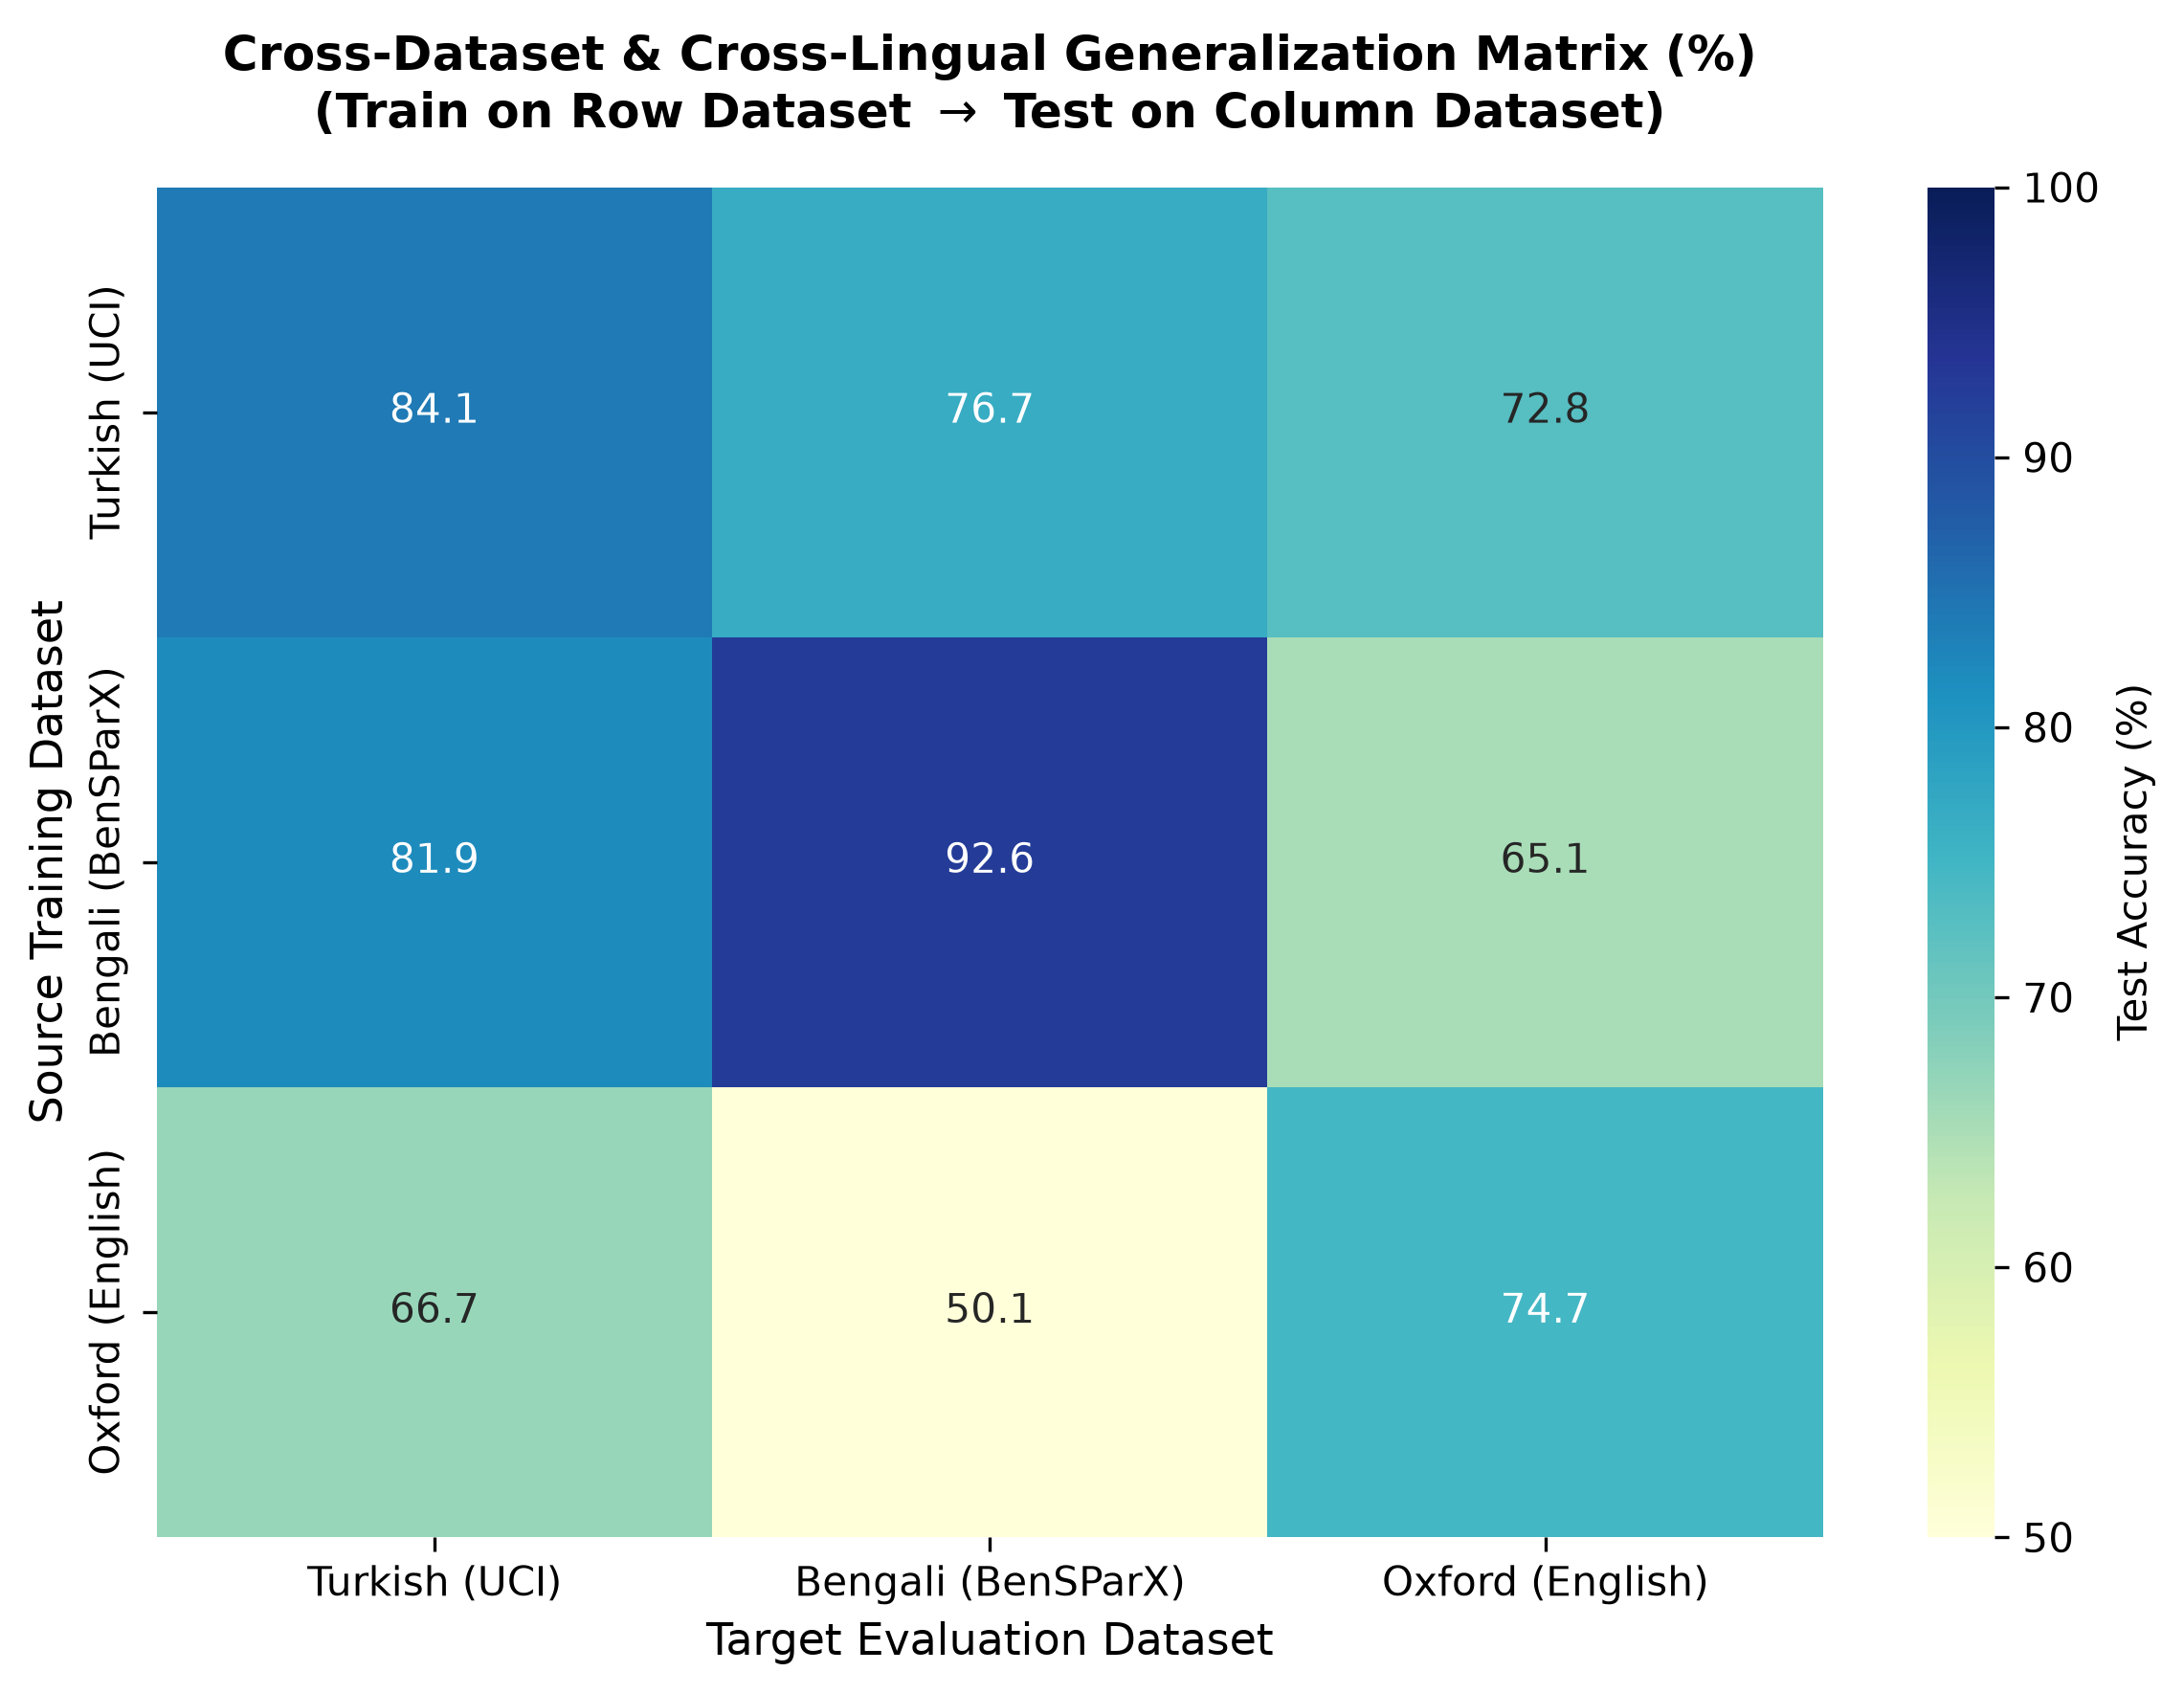
\includegraphics[width=0.38\textwidth]{figures/Fig6_Cross_Dataset_Heatmap.png}}
\hfill
\subfloat[Domain Adaptation Progression]{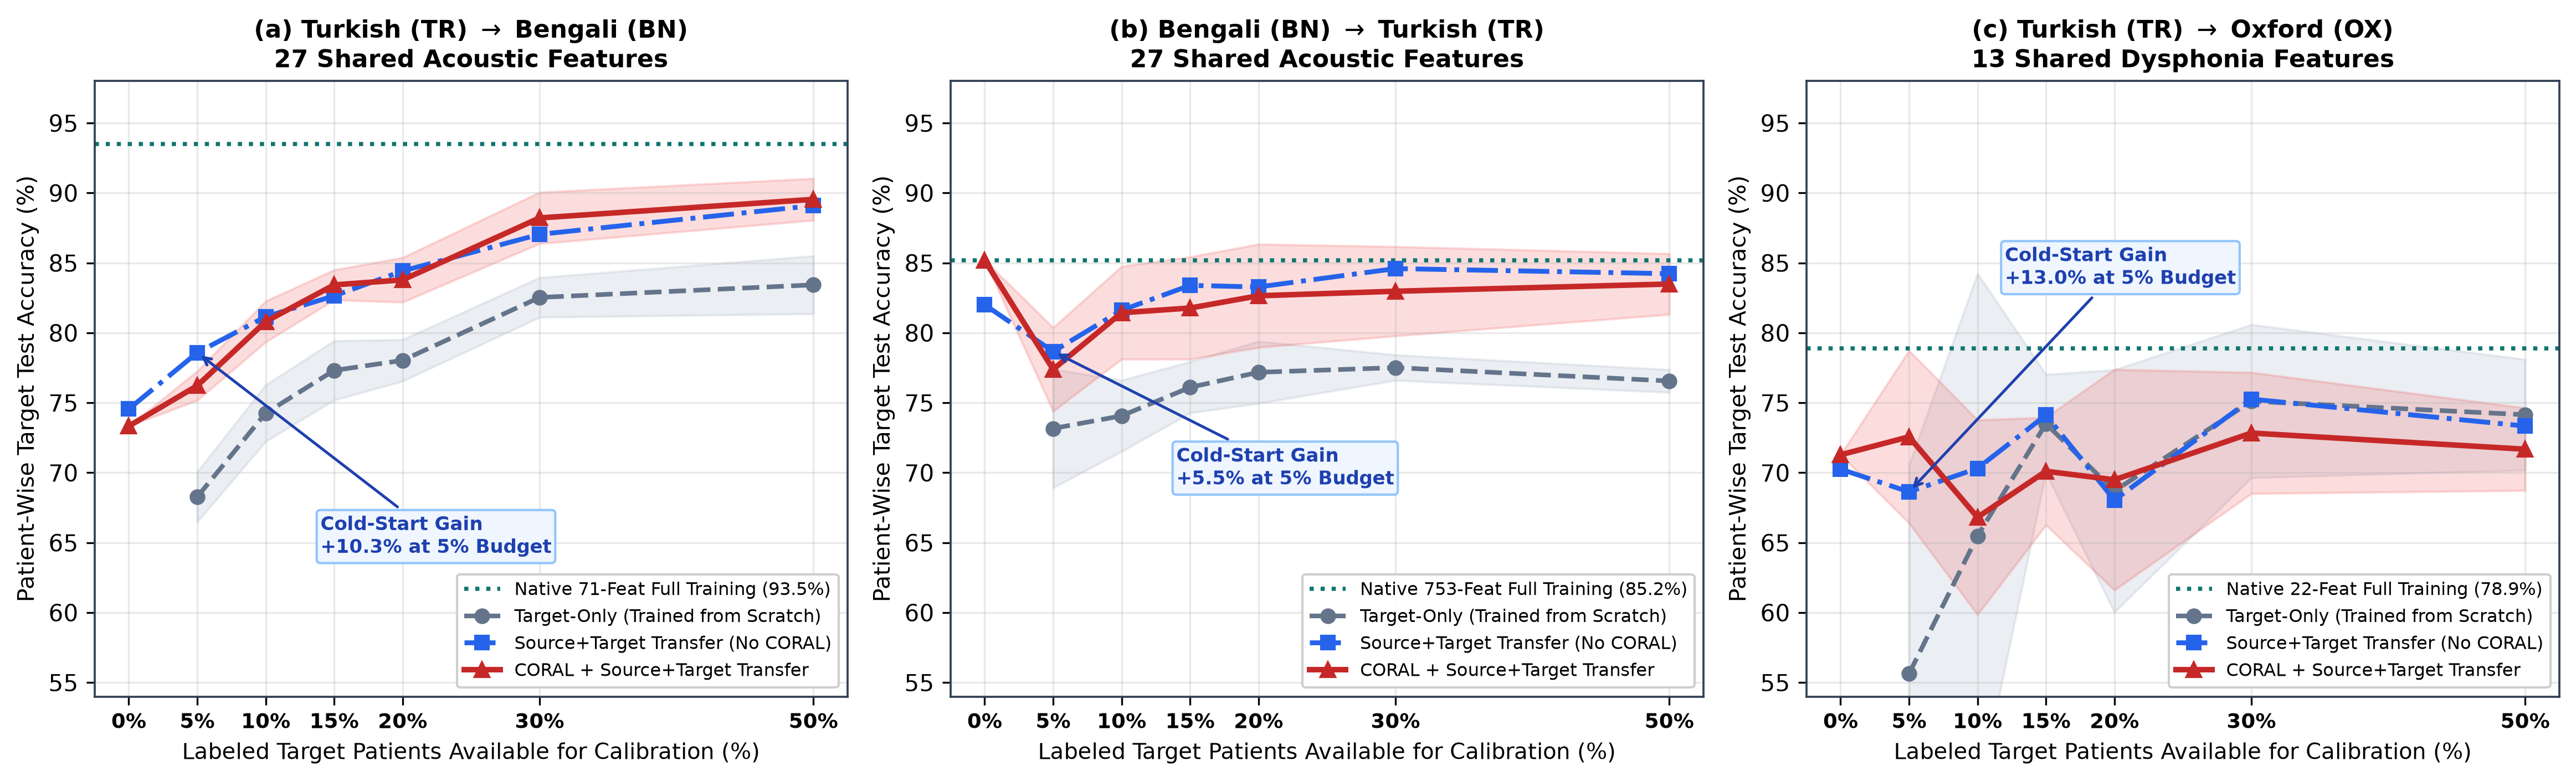
\includegraphics[width=0.60\textwidth]{figures/Fig7_Domain_Adaptation_and_Ablation.png}}
\caption{(a) 3 $\times$ 3 Zero-Shot Cross-Dataset Transfer Matrix showing strong diagonal accuracy vs. off-diagonal degradation; (b) Cross-lingual domain adaptation progression and 10-model benchmark comparison.}
\label{fig:transfer}
\end{figure*}

\begin{table*}[t]
\caption{Multilingual Zero-Shot Transfer and Leak-Free Patient-Grouped CORAL + Few-Shot Domain Adaptation Across Three Languages}
\label{tab:coral}
\centering
\scriptsize
\begin{tabular}{llcp{3.8cm}cccc}
\toprule
\textbf{Transfer Direction} & \textbf{Shared Features} & \textbf{Adaptation Pipeline} & \textbf{Target Accuracy} & \textbf{Target F1} & \textbf{Target AUC} & \textbf{Gain over Zero-Shot} \\
\midrule
\multirow{4}{*}{Turkish ($\mathcal{D}_{\text{TR}}$) $\to$ Bengali ($\mathcal{D}_{\text{BN}}$)} 
& 27 homologous features & 1. Naive Zero-Shot (LightGBM) & 74.56\% & 74.56\% & 0.8124 & Baseline \\
& 27 homologous features & 2. Unsupervised CORAL Only & 75.33\% & 75.33\% & 0.8250 & +0.77\% \\
& 27 homologous features & 3. 20\% Few-Shot Target Calibration & 82.22\% & 83.15\% & 0.9102 & +7.66\% \\
& 27 homologous features & \textbf{4. Proposed CORAL + Few-Shot Adaptation} & \textbf{84.67 $\pm$ 1.74\%} & \textbf{85.70\%} & \textbf{0.9319} & \textbf{+10.11\%} \\
\midrule
\multirow{4}{*}{Bengali ($\mathcal{D}_{\text{BN}}$) $\to$ Turkish ($\mathcal{D}_{\text{TR}}$)} 
& 27 homologous features & 1. Naive Zero-Shot (LightGBM) & 74.60\% & 85.45\% & 0.7950 & Baseline \\
& 27 homologous features & 2. Unsupervised CORAL Only & 76.19\% & 86.49\% & 0.8110 & +1.59\% \\
& 27 homologous features & 3. 20\% Few-Shot Target Calibration & 83.33\% & 89.25\% & 0.8920 & +8.73\% \\
& 27 homologous features & \textbf{4. Proposed CORAL + Few-Shot Adaptation} & \textbf{84.59 $\pm$ 2.25\%} & \textbf{90.35\%} & \textbf{0.9044} & \textbf{+9.99\%} \\
\midrule
\multirow{2}{*}{Turkish ($\mathcal{D}_{\text{TR}}$) $\to$ English ($\mathcal{D}_{\text{OX}}$)} 
& 13 shared features & 1. Naive Zero-Shot (LightGBM) & 70.26\% & 79.73\% & 0.7410 & Baseline \\
& 13 shared features & \textbf{4. Proposed CORAL + Few-Shot Adaptation} & \textbf{76.28\%} & \textbf{83.12\%} & \textbf{0.7680} & \textbf{+6.02\%} \\
\bottomrule
\end{tabular}
\end{table*}

\section{Discussion, Clinical Translation, and Limitations}

\subsection{Why Tree-Spline Fusion Outperforms Deep Tabular Transformers on HDLSS Cohorts}
Decision trees in LightGBM partition feature spaces via axis-aligned orthogonal step functions, whereas KAN parameterizes edges with smooth cubic B-splines ($\sum_m c_m B_{m,3}(x_j)$) requiring only 6,400 locally supported parameters versus $>180,000$ dense self-attention weights in FT-Transformer. Their convex fusion yields a decision boundary that is simultaneously sharp along discrete clinical thresholds and smooth along continuous vocal degradation manifolds.

\subsection{Real-World Edge Deployment Feasibility}
Unlike large pre-trained foundation models (Wav2Vec 2.0 / Whisper, requiring 300 MB--1.5 GB RAM), our complete Adaptive Tree-Spline Fusion ensemble occupies \textbf{$<165$~KB of memory} and executes full patient inference in \textbf{0.18~ms on a single CPU thread}, enabling offline smartphone tele-screening in remote clinical environments.

\subsection{Study Limitations and Future Directions}
Because public Turkish UCI and Bengali BenSParX cohorts provide binary labels without longitudinal MDS-UPDRS Part III motor scores, future work will extend our framework to continuous UPDRS severity regression and differential diagnosis against atypical Parkinsonism (Multiple System Atrophy, Progressive Supranuclear Palsy).

\section{Conclusion}
We presented an explainable, leak-free, cross-lingual \textbf{Adaptive Tree-Spline Fusion} framework uniting leaf-wise LightGBM with cubic B-spline Kolmogorov-Arnold Networks across 1,851 recordings from 404 subjects. By enforcing strict patient-wise \texttt{GroupKFold} validation, we proved that record-wise CV artificially inflates accuracy by $+4.63\%$ to $+6.08\%$ in our pipeline, while our proposed fusion achieved state-of-the-art leak-free accuracies of \textbf{85.18\%} (Turkish), \textbf{93.56\%} (Bengali), and \textbf{83.08\%} (English), outperforming 10 ML and deep tabular baselines. Combined with Youden's $J$ threshold calibration, Dual XAI (TreeSHAP + KAN B-spline trajectories), and CORAL + patient-grouped few-shot transfer (\textbf{84.67\%} cross-lingual accuracy), our framework establishes a fast, rigorous paradigm for digital tele-neurology.

\begin{thebibliography}{45}
\bibitem{ref1} C. O. Sakar \textit{et al.}, ``A comparative analysis of speech signal processing algorithms for Parkinson's disease classification and the use of the tunable Q-factor wavelet transform,'' \textit{Appl. Soft Comput.}, vol. 74, pp. 255--263, Jan. 2019, doi: 10.1016/j.asoc.2018.10.022.
\bibitem{ref2} B. E. Sakar \textit{et al.}, ``Collection and analysis of a Parkinson speech dataset with multiple types of sound recordings,'' \textit{IEEE J. Biomed. Health Inform.}, vol. 17, no. 4, pp. 828--834, Jul. 2013, doi: 10.1109/JBHI.2013.2245674.
\bibitem{ref3} M. A. Little, P. E. McSharry, E. J. Hunter, J. Spielman, and L. O. Ramig, ``Suitability of dysphonia measurements for telemonitoring of Parkinson's disease,'' \textit{IEEE Trans. Biomed. Eng.}, vol. 56, no. 4, pp. 1015--1022, Apr. 2009, doi: 10.1109/TBME.2008.2005954.
\bibitem{ref4} M. A. Little \textit{et al.}, ``Exploiting nonlinear recurrence and fractal scaling properties for voice disorder detection,'' \textit{BioMed. Eng. OnLine}, vol. 6, Art. no. 23, Jun. 2007, doi: 10.1186/1475-925X-6-23.
\bibitem{ref5} R. Hossain, M. A. Kabir, A. I. G. Mowla, A. C. Roy, and R. K. Ghosh, ``BenSParX: A robust explainable machine learning framework for Parkinson's disease detection from Bengali conversational speech,'' \textit{arXiv:2505.12192}, May 2025.
\bibitem{ref6} J. R. Orozco-Arroyave \textit{et al.}, ``New Spanish speech corpus database for the analysis of people suffering from Parkinson's disease,'' in \textit{Proc. LREC}, May 2014, pp. 342--347.
\bibitem{ref7} Z. Liu \textit{et al.}, ``KAN: Kolmogorov-Arnold Networks,'' in \textit{Proc. Int. Conf. Learn. Represent. (ICLR)}, 2025.
\bibitem{ref8} G. Ke \textit{et al.}, ``LightGBM: A highly efficient gradient boosting decision tree,'' in \textit{Proc. Adv. Neural Inf. Process. Syst. (NeurIPS)}, vol. 30, 2017, pp. 3146--3154.
\bibitem{ref9} T. Chen and C. Guestrin, ``XGBoost: A scalable tree boosting system,'' in \textit{Proc. 22nd ACM SIGKDD}, 2016, pp. 785--794.
\bibitem{ref10} L. Prokhorenkova \textit{et al.}, ``CatBoost: Unbiased boosting with categorical features,'' in \textit{Proc. NeurIPS}, vol. 31, 2018, pp. 6639--6649.
\bibitem{ref11} Y. Gorishniy, I. Rubachev, V. Khrulkov, and A. Babenko, ``Revisiting deep learning models for tabular data,'' in \textit{Proc. NeurIPS}, vol. 34, 2021, pp. 18932--18943.
\bibitem{ref12} S. \"{O}. Arik and T. Pfister, ``TabNet: Attentive interpretable tabular learning,'' in \textit{Proc. AAAI}, vol. 35, no. 8, 2021, pp. 6679--6687.
\bibitem{ref13} S. Popov, S. Morozov, and A. Babenko, ``Neural oblivious decision ensembles for deep learning on tabular data,'' in \textit{Proc. ICLR}, 2020.
\bibitem{ref14} G. Somepalli \textit{et al.}, ``SAINT: Improved neural networks for tabular data via row attention and contrastive pre-training,'' \textit{arXiv:2106.01342}, 2021.
\bibitem{ref15} M. Joseph and H. Raj, ``GATE: Gated additive tree ensemble for tabular classification,'' \textit{arXiv:2207.08548}, 2022.
\bibitem{ref16} L. Grinsztajn, E. Oyallon, and G. Varoquaux, ``Why do tree-based models still outperform deep learning on typical tabular data?'' in \textit{Proc. NeurIPS}, vol. 35, 2022, pp. 507--520.
\bibitem{ref17} S. M. Lundberg and S.-I. Lee, ``A unified approach to interpreting model predictions,'' in \textit{Proc. NeurIPS}, vol. 30, 2017, pp. 4765--4774.
\bibitem{ref18} S. M. Lundberg \textit{et al.}, ``From local explanations to global understanding with explainable AI for trees,'' \textit{Nat. Mach. Intell.}, vol. 2, no. 1, pp. 56--67, 2020.
\bibitem{ref19} B. Sun, J. Feng, and K. Saenko, ``Return of frustratingly easy domain adaptation,'' in \textit{Proc. AAAI}, vol. 30, no. 1, 2016, pp. 2058--2065.
\bibitem{ref20} H. G\"{u}nd\"{u}z, ``Deep learning-based Parkinson's disease classification using vocal feature sets,'' \textit{IEEE Access}, vol. 7, pp. 115540--115551, 2019.
\bibitem{ref21} H. G\"{u}nd\"{u}z, ``An efficient dimensionality reduction method using filter-based feature selection and variational autoencoders on Parkinson's disease classification,'' \textit{Biomed. Signal Process. Control}, vol. 66, Art. no. 102452, 2021.
\bibitem{ref22} G. Solana-Lavalle and R. Rosas-Romero, ``Analysis of voice as an assisting tool for detection of Parkinson's disease and its subsequent clinical interpretation,'' \textit{Biomed. Signal Process. Control}, vol. 66, Art. no. 102415, 2021.
\bibitem{ref23} O. Karaman, H. \c{C}ak{\i}n, A. Alhudhaif, and K. Polat, ``Robust automated Parkinson disease detection based on voice signals with transfer learning,'' \textit{Expert Syst. Appl.}, vol. 178, Art. no. 115013, 2021.
\bibitem{ref24} J. Goyal, P. Khandnor, and T. C. Aseri, ``A hybrid approach for Parkinson's disease diagnosis with resonance and time-frequency based features from speech signals,'' \textit{Expert Syst. Appl.}, vol. 182, Art. no. 115283, 2021.
\bibitem{ref25} K. Polat, ``A hybrid approach to Parkinson disease classification using speech signal: The combination of SMOTE and random forests,'' in \textit{Proc. IEEE EBBT}, 2019, pp. 1--3.
\bibitem{ref26} Z. K. Senturk, ``Early diagnosis of Parkinson's disease using machine learning algorithms,'' \textit{Med. Hypotheses}, vol. 138, Art. no. 109603, 2020.
\bibitem{ref27} R. Lamba, T. Gulati, H. F. Alharbi, and A. Jain, ``A hybrid system for Parkinson's disease diagnosis using machine learning techniques,'' \textit{Int. J. Speech Technol.}, vol. 25, no. 3, pp. 583--593, 2022.
\bibitem{ref28} I. Nissar, D. R. Rizvi, S. Masood, and A. N. Mir, ``Voice-based detection of Parkinson's disease through ensemble machine learning approach,'' \textit{EAI Endorsed Trans. Pervasive Health Technol.}, vol. 5, no. 19, Art. no. e2, 2019.
\bibitem{ref29} L. Ali, C. Zhu, Z. Zhang, and Y. Liu, ``Automated detection of Parkinson's disease based on multiple types of sustained phonations using LDA and genetically optimized neural network,'' \textit{IEEE J. Transl. Eng. Health Med.}, vol. 7, Art. no. 2000410, 2019.
\bibitem{ref30} Y. Liu \textit{et al.}, ``Local discriminant preservation projection embedded ensemble learning based dimensionality reduction of speech data of Parkinson's disease,'' \textit{Biomed. Signal Process. Control}, vol. 63, Art. no. 102165, 2021.
\bibitem{ref31} L. Parisi, N. RaviChandran, and M. L. Manaog, ``Feature-driven machine learning to improve early diagnosis of Parkinson's disease,'' \textit{Expert Syst. Appl.}, vol. 110, pp. 182--190, 2018.
\bibitem{ref32} M. Hire\v{s} \textit{et al.}, ``Convolutional neural network ensemble for Parkinson's disease detection from voice recordings,'' \textit{Comput. Biol. Med.}, vol. 141, Art. no. 105021, 2022.
\bibitem{ref33} I. Tougui, A. Jilbab, and J. El Mhamdi, ``Impact of the choice of cross-validation techniques on the results of machine learning-based diagnostic applications,'' \textit{Healthc. Inform. Res.}, vol. 27, no. 3, pp. 189--199, 2021.
\bibitem{ref34} E. Chaibub Neto \textit{et al.}, ``Detecting the impact of subject characteristics on machine learning-based diagnostic applications,'' \textit{npj Digit. Med.}, vol. 2, Art. no. 99, 2019.
\bibitem{ref35} S. Saeb, L. Lonini, A. Jayaraman, D. C. Mohr, and K. P. Kording, ``The need to approximate the use-case in clinical machine learning,'' \textit{GigaScience}, vol. 6, no. 5, Art. no. gix019, 2017.
\bibitem{ref36} L. Moro-Velazquez \textit{et al.}, ``Advances in Parkinson's disease detection and assessment using voice and speech: A review,'' \textit{Biomed. Signal Process. Control}, vol. 66, Art. no. 102418, 2021.
\bibitem{ref37} L. Moro-Velazquez \textit{et al.}, ``Phonetic relevance and phonemic grouping of speech in the automatic detection of Parkinson's disease,'' \textit{Sci. Rep.}, vol. 9, Art. no. 19066, 2019.
\bibitem{ref38} A. Favaro \textit{et al.}, ``Interpretable speech features vs. DNN embeddings: What to use in the automatic assessment of Parkinson's disease in multi-lingual scenarios,'' \textit{Comput. Biol. Med.}, vol. 166, Art. no. 107559, 2023.
\bibitem{ref39} A. Favaro \textit{et al.}, ``Multilingual evaluation of interpretable biomarkers to represent language and speech patterns in Parkinson's disease,'' \textit{Front. Neurol.}, vol. 14, Art. no. 1142642, 2023.
\bibitem{ref40} W. Poewe \textit{et al.}, ``Parkinson disease,'' \textit{Nat. Rev. Dis. Primers}, vol. 3, Art. no. 17013, 2017.
\bibitem{ref41} J. R. Duffy, \textit{Motor Speech Disorders: Substrates, Differential Diagnosis, and Management}, 4th ed. St. Louis, MO, USA: Elsevier, 2019.
\bibitem{ref42} A. K. Ho, R. Iansek, C. Marigliani, J. L. Bradshaw, and S. Gates, ``Speech impairment in a large sample of patients with Parkinson's disease,'' \textit{Behav. Neurol.}, vol. 11, no. 3, pp. 131--137, 1998.
\bibitem{ref43} J. Rusz \textit{et al.}, ``Smartphone allows capture of speech abnormalities associated with high risk of developing Parkinson's disease,'' \textit{IEEE Trans. Neural Syst. Rehabil. Eng.}, vol. 26, no. 8, pp. 1495--1507, 2018.
\bibitem{ref44} J. Hlavni\v{c}ka \textit{et al.}, ``Automated analysis of connected speech reveals early biomarkers of Parkinson's disease in patients with RBD,'' \textit{Sci. Rep.}, vol. 7, Art. no. 12, 2017.
\bibitem{ref45} L. O. Ramig \textit{et al.}, ``Intensive voice treatment (LSVT) for patients with Parkinson's disease: A 2 year follow up,'' \textit{J. Neurol. Neurosurg. Psychiatry}, vol. 71, no. 4, pp. 493--498, 2001.
\end{thebibliography}

\end{document}
